% Options for packages loaded elsewhere
% Options for packages loaded elsewhere
\PassOptionsToPackage{unicode}{hyperref}
\PassOptionsToPackage{hyphens}{url}
\PassOptionsToPackage{dvipsnames,svgnames,x11names}{xcolor}
%
\documentclass[
  letterpaper,
  DIV=11,
  numbers=noendperiod]{scrreprt}
\usepackage{xcolor}
\usepackage{amsmath,amssymb}
\setcounter{secnumdepth}{5}
\usepackage{iftex}
\ifPDFTeX
  \usepackage[T1]{fontenc}
  \usepackage[utf8]{inputenc}
  \usepackage{textcomp} % provide euro and other symbols
\else % if luatex or xetex
  \usepackage{unicode-math} % this also loads fontspec
  \defaultfontfeatures{Scale=MatchLowercase}
  \defaultfontfeatures[\rmfamily]{Ligatures=TeX,Scale=1}
\fi
\usepackage{lmodern}
\ifPDFTeX\else
  % xetex/luatex font selection
\fi
% Use upquote if available, for straight quotes in verbatim environments
\IfFileExists{upquote.sty}{\usepackage{upquote}}{}
\IfFileExists{microtype.sty}{% use microtype if available
  \usepackage[]{microtype}
  \UseMicrotypeSet[protrusion]{basicmath} % disable protrusion for tt fonts
}{}
\makeatletter
\@ifundefined{KOMAClassName}{% if non-KOMA class
  \IfFileExists{parskip.sty}{%
    \usepackage{parskip}
  }{% else
    \setlength{\parindent}{0pt}
    \setlength{\parskip}{6pt plus 2pt minus 1pt}}
}{% if KOMA class
  \KOMAoptions{parskip=half}}
\makeatother
% Make \paragraph and \subparagraph free-standing
\makeatletter
\ifx\paragraph\undefined\else
  \let\oldparagraph\paragraph
  \renewcommand{\paragraph}{
    \@ifstar
      \xxxParagraphStar
      \xxxParagraphNoStar
  }
  \newcommand{\xxxParagraphStar}[1]{\oldparagraph*{#1}\mbox{}}
  \newcommand{\xxxParagraphNoStar}[1]{\oldparagraph{#1}\mbox{}}
\fi
\ifx\subparagraph\undefined\else
  \let\oldsubparagraph\subparagraph
  \renewcommand{\subparagraph}{
    \@ifstar
      \xxxSubParagraphStar
      \xxxSubParagraphNoStar
  }
  \newcommand{\xxxSubParagraphStar}[1]{\oldsubparagraph*{#1}\mbox{}}
  \newcommand{\xxxSubParagraphNoStar}[1]{\oldsubparagraph{#1}\mbox{}}
\fi
\makeatother

\usepackage{color}
\usepackage{fancyvrb}
\newcommand{\VerbBar}{|}
\newcommand{\VERB}{\Verb[commandchars=\\\{\}]}
\DefineVerbatimEnvironment{Highlighting}{Verbatim}{commandchars=\\\{\}}
% Add ',fontsize=\small' for more characters per line
\usepackage{framed}
\definecolor{shadecolor}{RGB}{241,243,245}
\newenvironment{Shaded}{\begin{snugshade}}{\end{snugshade}}
\newcommand{\AlertTok}[1]{\textcolor[rgb]{0.68,0.00,0.00}{#1}}
\newcommand{\AnnotationTok}[1]{\textcolor[rgb]{0.37,0.37,0.37}{#1}}
\newcommand{\AttributeTok}[1]{\textcolor[rgb]{0.40,0.45,0.13}{#1}}
\newcommand{\BaseNTok}[1]{\textcolor[rgb]{0.68,0.00,0.00}{#1}}
\newcommand{\BuiltInTok}[1]{\textcolor[rgb]{0.00,0.23,0.31}{#1}}
\newcommand{\CharTok}[1]{\textcolor[rgb]{0.13,0.47,0.30}{#1}}
\newcommand{\CommentTok}[1]{\textcolor[rgb]{0.37,0.37,0.37}{#1}}
\newcommand{\CommentVarTok}[1]{\textcolor[rgb]{0.37,0.37,0.37}{\textit{#1}}}
\newcommand{\ConstantTok}[1]{\textcolor[rgb]{0.56,0.35,0.01}{#1}}
\newcommand{\ControlFlowTok}[1]{\textcolor[rgb]{0.00,0.23,0.31}{\textbf{#1}}}
\newcommand{\DataTypeTok}[1]{\textcolor[rgb]{0.68,0.00,0.00}{#1}}
\newcommand{\DecValTok}[1]{\textcolor[rgb]{0.68,0.00,0.00}{#1}}
\newcommand{\DocumentationTok}[1]{\textcolor[rgb]{0.37,0.37,0.37}{\textit{#1}}}
\newcommand{\ErrorTok}[1]{\textcolor[rgb]{0.68,0.00,0.00}{#1}}
\newcommand{\ExtensionTok}[1]{\textcolor[rgb]{0.00,0.23,0.31}{#1}}
\newcommand{\FloatTok}[1]{\textcolor[rgb]{0.68,0.00,0.00}{#1}}
\newcommand{\FunctionTok}[1]{\textcolor[rgb]{0.28,0.35,0.67}{#1}}
\newcommand{\ImportTok}[1]{\textcolor[rgb]{0.00,0.46,0.62}{#1}}
\newcommand{\InformationTok}[1]{\textcolor[rgb]{0.37,0.37,0.37}{#1}}
\newcommand{\KeywordTok}[1]{\textcolor[rgb]{0.00,0.23,0.31}{\textbf{#1}}}
\newcommand{\NormalTok}[1]{\textcolor[rgb]{0.00,0.23,0.31}{#1}}
\newcommand{\OperatorTok}[1]{\textcolor[rgb]{0.37,0.37,0.37}{#1}}
\newcommand{\OtherTok}[1]{\textcolor[rgb]{0.00,0.23,0.31}{#1}}
\newcommand{\PreprocessorTok}[1]{\textcolor[rgb]{0.68,0.00,0.00}{#1}}
\newcommand{\RegionMarkerTok}[1]{\textcolor[rgb]{0.00,0.23,0.31}{#1}}
\newcommand{\SpecialCharTok}[1]{\textcolor[rgb]{0.37,0.37,0.37}{#1}}
\newcommand{\SpecialStringTok}[1]{\textcolor[rgb]{0.13,0.47,0.30}{#1}}
\newcommand{\StringTok}[1]{\textcolor[rgb]{0.13,0.47,0.30}{#1}}
\newcommand{\VariableTok}[1]{\textcolor[rgb]{0.07,0.07,0.07}{#1}}
\newcommand{\VerbatimStringTok}[1]{\textcolor[rgb]{0.13,0.47,0.30}{#1}}
\newcommand{\WarningTok}[1]{\textcolor[rgb]{0.37,0.37,0.37}{\textit{#1}}}

\usepackage{longtable,booktabs,array}
\usepackage{calc} % for calculating minipage widths
% Correct order of tables after \paragraph or \subparagraph
\usepackage{etoolbox}
\makeatletter
\patchcmd\longtable{\par}{\if@noskipsec\mbox{}\fi\par}{}{}
\makeatother
% Allow footnotes in longtable head/foot
\IfFileExists{footnotehyper.sty}{\usepackage{footnotehyper}}{\usepackage{footnote}}
\makesavenoteenv{longtable}
\usepackage{graphicx}
\makeatletter
\newsavebox\pandoc@box
\newcommand*\pandocbounded[1]{% scales image to fit in text height/width
  \sbox\pandoc@box{#1}%
  \Gscale@div\@tempa{\textheight}{\dimexpr\ht\pandoc@box+\dp\pandoc@box\relax}%
  \Gscale@div\@tempb{\linewidth}{\wd\pandoc@box}%
  \ifdim\@tempb\p@<\@tempa\p@\let\@tempa\@tempb\fi% select the smaller of both
  \ifdim\@tempa\p@<\p@\scalebox{\@tempa}{\usebox\pandoc@box}%
  \else\usebox{\pandoc@box}%
  \fi%
}
% Set default figure placement to htbp
\def\fps@figure{htbp}
\makeatother





\setlength{\emergencystretch}{3em} % prevent overfull lines

\providecommand{\tightlist}{%
  \setlength{\itemsep}{0pt}\setlength{\parskip}{0pt}}



 


\KOMAoption{captions}{tableheading}
\makeatletter
\@ifpackageloaded{bookmark}{}{\usepackage{bookmark}}
\makeatother
\makeatletter
\@ifpackageloaded{caption}{}{\usepackage{caption}}
\AtBeginDocument{%
\ifdefined\contentsname
  \renewcommand*\contentsname{Table of contents}
\else
  \newcommand\contentsname{Table of contents}
\fi
\ifdefined\listfigurename
  \renewcommand*\listfigurename{List of Figures}
\else
  \newcommand\listfigurename{List of Figures}
\fi
\ifdefined\listtablename
  \renewcommand*\listtablename{List of Tables}
\else
  \newcommand\listtablename{List of Tables}
\fi
\ifdefined\figurename
  \renewcommand*\figurename{Figure}
\else
  \newcommand\figurename{Figure}
\fi
\ifdefined\tablename
  \renewcommand*\tablename{Table}
\else
  \newcommand\tablename{Table}
\fi
}
\@ifpackageloaded{float}{}{\usepackage{float}}
\floatstyle{ruled}
\@ifundefined{c@chapter}{\newfloat{codelisting}{h}{lop}}{\newfloat{codelisting}{h}{lop}[chapter]}
\floatname{codelisting}{Listing}
\newcommand*\listoflistings{\listof{codelisting}{List of Listings}}
\makeatother
\makeatletter
\makeatother
\makeatletter
\@ifpackageloaded{caption}{}{\usepackage{caption}}
\@ifpackageloaded{subcaption}{}{\usepackage{subcaption}}
\makeatother
\usepackage{bookmark}
\IfFileExists{xurl.sty}{\usepackage{xurl}}{} % add URL line breaks if available
\urlstyle{same}
\hypersetup{
  pdftitle={Оценка водных биоресурсов при недостатке данных в среде R (для начинающих)},
  pdfauthor={Сергей Баканёв},
  colorlinks=true,
  linkcolor={blue},
  filecolor={Maroon},
  citecolor={Blue},
  urlcolor={Blue},
  pdfcreator={LaTeX via pandoc}}


\title{Оценка водных биоресурсов при недостатке данных в среде R (для
начинающих)}
\author{Сергей Баканёв}
\date{2025-04-30}
\begin{document}
\maketitle

\renewcommand*\contentsname{Table of contents}
{
\hypersetup{linkcolor=}
\setcounter{tocdepth}{2}
\tableofcontents
}

\bookmarksetup{startatroot}

\chapter*{Аннотация}\label{ux430ux43dux43dux43eux442ux430ux446ux438ux44f}
\addcontentsline{toc}{chapter}{Аннотация}

\markboth{Аннотация}{Аннотация}

\textbf{Баканев С. В. (2025) Оценка водных биоресурсов при недостатке
данных в среде R (для начинающих). --- Курс лекций и практических
занятий, адрес доступа:~https://mombus.github.io/cRab}

Здесь будет краткая аннотация.

\bookmarksetup{startatroot}

\chapter{Введение}\label{ux432ux432ux435ux434ux435ux43dux438ux435}

В эпоху больших языковых моделей (LLM) вопрос об актуальности создания
структурированных учебников кажется закономерным. Зачем тратить время на
детальную проработку курса, если современные инструменты способны быстро
сгенерировать объяснение даже сложных тем --- от статистических формул
до методов оценки запасов? Однако многолетний опыт работы с
количественными данными в морской биологии подсказывает: формальные
алгоритмы не заменят практического понимания, необходимого для адаптации
теоретических подходов к реальным условиям.

LLM могут описать формулу Бейеса или работу программного обеспечения для
оценки запасов, но они не научат учитывать специфику конкретного региона
--- например, как интерпретировать противоречивые данные с научных
съемок или корректировать модели в условиях изменяющегося климата.
Именно в таких ситуациях ключевую роль играет опыт: годы наблюдений,
анализ ошибок и постепенная выработка гибких подходов к решению задач.

Этот репозиторий --- собрание проверенных методов, применявшихся при
решении прикладных задач: от обработки данных CPUE при неполном покрытии
акватории до моделирования распространения инвазивных видов с учетом
геоморфологических особенностей. Здесь вы найдете примеры, редко
встречающиеся в общедоступных источниках: как работать с
фрагментированными биотопами или оценивать сдвиги в ареалах видов на
основе долгосрочных наблюдений.

Большие языковые модели --- полезный инструмент, но их ответы часто
абстрактны. Реальная работа с данными требует не только технических
навыков, но и умения адаптироваться к уникальным условиям, где
неопределенность --- норма, а решения рождаются через анализ конкретных
случаев. Этот учебник направлен на передачу именно такого «живого»
опыта, который невозможно заменить автоматически сгенерированными
текстами.

\bookmarksetup{startatroot}

\chapter{Анализ и визуализация данных
улова}\label{ux430ux43dux430ux43bux438ux437-ux438-ux432ux438ux437ux443ux430ux43bux438ux437ux430ux446ux438ux44f-ux434ux430ux43dux43dux44bux445-ux443ux43bux43eux432ux430}

\section{Введение (в
R)}\label{ux432ux432ux435ux434ux435ux43dux438ux435-ux432-r}

\section{Загрузка данных и первичный
осмотр}\label{ux437ux430ux433ux440ux443ux437ux43aux430-ux434ux430ux43dux43dux44bux445-ux438-ux43fux435ux440ux432ux438ux447ux43dux44bux439-ux43eux441ux43cux43eux442ux440}

ссылка на файл:
\href{https://mombus.github.io/cRab/data/shrimp_catch.csv}{shrimp\_catch.csv}

\begin{Shaded}
\begin{Highlighting}[]
\CommentTok{\# Установка рабочей директории}
\FunctionTok{setwd}\NormalTok{(}\StringTok{"C:/TEXTBOOK/"}\NormalTok{)}
\CommentTok{\# Загрузка библиотек}
\FunctionTok{library}\NormalTok{(tidyverse)}
\CommentTok{\# Загрузка данных}
\NormalTok{data }\OtherTok{\textless{}{-}} \FunctionTok{read\_csv}\NormalTok{(}\StringTok{"shrimp\_catch.csv"}\NormalTok{)}
\end{Highlighting}
\end{Shaded}

Команда \texttt{glimpse} знакомит со структурой данных:

\begin{Shaded}
\begin{Highlighting}[]
\CommentTok{\# Просмотр структуры и первых строк загруженных данных}
\FunctionTok{glimpse}\NormalTok{(data)}
\end{Highlighting}
\end{Shaded}

\begin{Shaded}
\begin{Highlighting}[]
\NormalTok{Rows}\SpecialCharTok{:} \DecValTok{230}
\NormalTok{Columns}\SpecialCharTok{:} \DecValTok{5}
\SpecialCharTok{$}\NormalTok{ id     }\SpecialCharTok{\textless{}}\NormalTok{int}\SpecialCharTok{\textgreater{}} \DecValTok{1}\NormalTok{, }\DecValTok{2}\NormalTok{, }\DecValTok{3}\NormalTok{, }\DecValTok{4}\NormalTok{, }\DecValTok{5}\NormalTok{, }\DecValTok{6}\NormalTok{, }\DecValTok{7}\NormalTok{, }\DecValTok{8}\NormalTok{, }\DecValTok{9}\NormalTok{, }\DecValTok{10}\NormalTok{, }\DecValTok{11}\NormalTok{, }\DecValTok{12}\NormalTok{, }\DecValTok{13}\NormalTok{, }\DecValTok{14}\NormalTok{, }\DecValTok{15}\NormalTok{, }\DecValTok{16}\NormalTok{, }\DecValTok{17}\NormalTok{, }\DecValTok{18}\NormalTok{, }\SpecialCharTok{\textasciitilde{}}
\ErrorTok{$}\NormalTok{ age    }\SpecialCharTok{\textless{}}\NormalTok{int}\SpecialCharTok{\textgreater{}} \DecValTok{2}\NormalTok{, }\DecValTok{4}\NormalTok{, }\DecValTok{4}\NormalTok{, }\DecValTok{4}\NormalTok{, }\DecValTok{1}\NormalTok{, }\DecValTok{4}\NormalTok{, }\DecValTok{2}\NormalTok{, }\DecValTok{2}\NormalTok{, }\DecValTok{4}\NormalTok{, }\DecValTok{3}\NormalTok{, }\DecValTok{4}\NormalTok{, }\DecValTok{3}\NormalTok{, }\DecValTok{2}\NormalTok{, }\DecValTok{1}\NormalTok{, }\DecValTok{2}\NormalTok{, }\DecValTok{1}\NormalTok{, }\DecValTok{2}\NormalTok{, }\DecValTok{2}\NormalTok{, }\DecValTok{2}\NormalTok{, }\DecValTok{2}\NormalTok{, }\DecValTok{3}\NormalTok{, }\SpecialCharTok{\textasciitilde{}}
\ErrorTok{$}\NormalTok{ length }\SpecialCharTok{\textless{}}\NormalTok{dbl}\SpecialCharTok{\textgreater{}} \FloatTok{20.45450}\NormalTok{, }\FloatTok{25.88928}\NormalTok{, }\FloatTok{29.42257}\NormalTok{, }\FloatTok{30.68292}\NormalTok{, }\FloatTok{12.46059}\NormalTok{, }\FloatTok{28.52152}\NormalTok{, }\FloatTok{17.}\SpecialCharTok{\textasciitilde{}}
\ErrorTok{$}\NormalTok{ weight }\SpecialCharTok{\textless{}}\NormalTok{dbl}\SpecialCharTok{\textgreater{}} \FloatTok{1.28221748}\NormalTok{, }\FloatTok{1.97476899}\NormalTok{, }\FloatTok{2.65412595}\NormalTok{, }\FloatTok{3.44746476}\NormalTok{, }\FloatTok{0.13404801}\NormalTok{, }\FloatTok{2.3}\SpecialCharTok{\textasciitilde{}}
\ErrorTok{$}\NormalTok{ sex    }\SpecialCharTok{\textless{}}\NormalTok{chr}\SpecialCharTok{\textgreater{}} \StringTok{"M"}\NormalTok{, }\StringTok{"F"}\NormalTok{, }\StringTok{"F"}\NormalTok{, }\StringTok{"F"}\NormalTok{, }\StringTok{"M"}\NormalTok{, }\StringTok{"F"}\NormalTok{, }\StringTok{"M"}\NormalTok{, }\StringTok{"M"}\NormalTok{, }\StringTok{"F"}\NormalTok{, }\StringTok{"F"}\NormalTok{, }\StringTok{"F"}\NormalTok{, }\StringTok{"F"}\NormalTok{, }\StringTok{"M"}\SpecialCharTok{\textasciitilde{}}
\ErrorTok{\textgreater{}} 
\end{Highlighting}
\end{Shaded}

Можно использовать команду \texttt{str} --- показывает внутреннюю
\textbf{структуру} объекта , включая количество строк, столбцов,
названия переменных, их типы (\texttt{chr}, \texttt{num}, \texttt{int} и
др.), а также несколько первых значений.

\begin{Shaded}
\begin{Highlighting}[]
\FunctionTok{str}\NormalTok{(data)}
\end{Highlighting}
\end{Shaded}

\begin{Shaded}
\begin{Highlighting}[]
\StringTok{\textquotesingle{}data.frame\textquotesingle{}}\SpecialCharTok{:}   \DecValTok{230}\NormalTok{ obs. of  }\DecValTok{5}\NormalTok{ variables}\SpecialCharTok{:}
 \ErrorTok{$}\NormalTok{ id    }\SpecialCharTok{:}\NormalTok{ int  }\DecValTok{1} \DecValTok{2} \DecValTok{3} \DecValTok{4} \DecValTok{5} \DecValTok{6} \DecValTok{7} \DecValTok{8} \DecValTok{9} \DecValTok{10}\NormalTok{ ...}
 \SpecialCharTok{$}\NormalTok{ age   }\SpecialCharTok{:}\NormalTok{ int  }\DecValTok{2} \DecValTok{4} \DecValTok{4} \DecValTok{4} \DecValTok{1} \DecValTok{4} \DecValTok{2} \DecValTok{2} \DecValTok{4} \DecValTok{3}\NormalTok{ ...}
 \SpecialCharTok{$}\NormalTok{ length}\SpecialCharTok{:}\NormalTok{ num  }\FloatTok{20.5} \FloatTok{25.9} \FloatTok{29.4} \FloatTok{30.7} \FloatTok{12.5}\NormalTok{ ...}
 \SpecialCharTok{$}\NormalTok{ weight}\SpecialCharTok{:}\NormalTok{ num  }\FloatTok{1.282} \FloatTok{1.975} \FloatTok{2.654} \FloatTok{3.447} \FloatTok{0.134}\NormalTok{ ...}
 \SpecialCharTok{$}\NormalTok{ sex   }\SpecialCharTok{:}\NormalTok{ chr  }\StringTok{"M"} \StringTok{"F"} \StringTok{"F"} \StringTok{"F"}\NormalTok{ ...}
\SpecialCharTok{\textgreater{}}
\end{Highlighting}
\end{Shaded}

\section{Описательная статистика и
визуализация}\label{ux43eux43fux438ux441ux430ux442ux435ux43bux44cux43dux430ux44f-ux441ux442ux430ux442ux438ux441ux442ux438ux43aux430-ux438-ux432ux438ux437ux443ux430ux43bux438ux437ux430ux446ux438ux44f}

Команда \texttt{summary} выводит \textbf{описательную статистику} для
каждой числовой переменной: минимум, 1-й квартиль, медиана, среднее, 3-й
квартиль, максимум; для категориальных переменных --- частоты.

\begin{Shaded}
\begin{Highlighting}[]
\CommentTok{\# Общая статистика}
\FunctionTok{summary}\NormalTok{(data)}
\end{Highlighting}
\end{Shaded}

\begin{Shaded}
\begin{Highlighting}[]
\NormalTok{       id              age            length          weight       }
\NormalTok{ Min.   }\SpecialCharTok{:}  \FloatTok{1.00}\NormalTok{   Min.   }\SpecialCharTok{:}\FloatTok{1.000}\NormalTok{   Min.   }\SpecialCharTok{:} \FloatTok{7.65}\NormalTok{   Min.   }\SpecialCharTok{:{-}}\FloatTok{0.3334}  
 \DecValTok{1}\NormalTok{st Qu.}\SpecialCharTok{:} \FloatTok{58.25}   \DecValTok{1}\NormalTok{st Qu.}\SpecialCharTok{:}\FloatTok{2.000}   \DecValTok{1}\NormalTok{st Qu.}\SpecialCharTok{:}\FloatTok{17.62}   \DecValTok{1}\NormalTok{st Qu.}\SpecialCharTok{:} \FloatTok{0.6320}  
\NormalTok{ Median }\SpecialCharTok{:}\FloatTok{115.50}\NormalTok{   Median }\SpecialCharTok{:}\FloatTok{3.000}\NormalTok{   Median }\SpecialCharTok{:}\FloatTok{22.49}\NormalTok{   Median }\SpecialCharTok{:} \FloatTok{1.3660}  
\NormalTok{ Mean   }\SpecialCharTok{:}\FloatTok{115.50}\NormalTok{   Mean   }\SpecialCharTok{:}\FloatTok{2.509}\NormalTok{   Mean   }\SpecialCharTok{:}\FloatTok{21.68}\NormalTok{   Mean   }\SpecialCharTok{:} \FloatTok{1.4933}  
 \DecValTok{3}\NormalTok{rd Qu.}\SpecialCharTok{:}\FloatTok{172.75}   \DecValTok{3}\NormalTok{rd Qu.}\SpecialCharTok{:}\FloatTok{3.000}   \DecValTok{3}\NormalTok{rd Qu.}\SpecialCharTok{:}\FloatTok{26.03}   \DecValTok{3}\NormalTok{rd Qu.}\SpecialCharTok{:} \FloatTok{2.1148}  
\NormalTok{ Max.   }\SpecialCharTok{:}\FloatTok{230.00}\NormalTok{   Max.   }\SpecialCharTok{:}\FloatTok{4.000}\NormalTok{   Max.   }\SpecialCharTok{:}\FloatTok{36.02}\NormalTok{   Max.   }\SpecialCharTok{:} \FloatTok{5.1316}  
\NormalTok{     sex           }
\NormalTok{ Length}\SpecialCharTok{:}\DecValTok{230}        
\NormalTok{ Class }\SpecialCharTok{:}\NormalTok{character  }
\NormalTok{ Mode  }\SpecialCharTok{:}\NormalTok{character  }
\end{Highlighting}
\end{Shaded}

Простейшими командами можно вычислить, например, соотоношение полов или
корреляцию длина-вес.

\begin{Shaded}
\begin{Highlighting}[]
\CommentTok{\# Соотношение полов}
\FunctionTok{prop.table}\NormalTok{(}\FunctionTok{table}\NormalTok{(data}\SpecialCharTok{$}\NormalTok{sex)) }\SpecialCharTok{\%\textgreater{}\%} \FunctionTok{round}\NormalTok{(}\DecValTok{2}\NormalTok{)}
\end{Highlighting}
\end{Shaded}

\begin{Shaded}
\begin{Highlighting}[]
\NormalTok{   F    M }
\FloatTok{0.35} \FloatTok{0.65} 
\end{Highlighting}
\end{Shaded}

\begin{Shaded}
\begin{Highlighting}[]
\CommentTok{\# Корреляция длина{-}вес с p{-}value}
\NormalTok{cor\_test }\OtherTok{\textless{}{-}} \FunctionTok{cor.test}\NormalTok{(data}\SpecialCharTok{$}\NormalTok{length, data}\SpecialCharTok{$}\NormalTok{weight, }
                     \AttributeTok{method =} \StringTok{"pearson"}\NormalTok{, }
                     \AttributeTok{exact =} \ConstantTok{FALSE}\NormalTok{,}
                     \AttributeTok{na.action =}\NormalTok{ na.omit)}
 
\NormalTok{cor\_coef }\OtherTok{\textless{}{-}} \FunctionTok{round}\NormalTok{(cor\_test}\SpecialCharTok{$}\NormalTok{estimate, }\DecValTok{2}\NormalTok{)}
\NormalTok{p\_value }\OtherTok{\textless{}{-}}\NormalTok{ scales}\SpecialCharTok{::}\FunctionTok{pvalue}\NormalTok{(cor\_test}\SpecialCharTok{$}\NormalTok{p.value, }\AttributeTok{accuracy =}\NormalTok{ .}\DecValTok{001}\NormalTok{)}
 
\FunctionTok{cat}\NormalTok{(}\StringTok{"Корреляция Пирсона: r ="}\NormalTok{, cor\_coef, }\StringTok{", p ="}\NormalTok{, p\_value, }\StringTok{"}\SpecialCharTok{\textbackslash{}n}\StringTok{"}\NormalTok{)}
\end{Highlighting}
\end{Shaded}

\begin{Shaded}
\begin{Highlighting}[]
\NormalTok{Корреляция Пирсона}\SpecialCharTok{:}\NormalTok{ r }\OtherTok{=} \FloatTok{0.95}\NormalTok{ , p }\OtherTok{=} \ErrorTok{\textless{}}\FloatTok{0.001} 
\end{Highlighting}
\end{Shaded}

\begin{Shaded}
\begin{Highlighting}[]
\CommentTok{\# Распределение возраста}
\FunctionTok{table}\NormalTok{(data}\SpecialCharTok{$}\NormalTok{age)}
\end{Highlighting}
\end{Shaded}

\begin{Shaded}
\begin{Highlighting}[]
\DecValTok{1}  \DecValTok{2}  \DecValTok{3}  \DecValTok{4} 
\DecValTok{43} \DecValTok{68} \DecValTok{77} \DecValTok{40} 
\end{Highlighting}
\end{Shaded}

\begin{Shaded}
\begin{Highlighting}[]
\CommentTok{\# Средние значения длины и веса по группам}
\NormalTok{data }\SpecialCharTok{\%\textgreater{}\%}
   \FunctionTok{group\_by}\NormalTok{(age) }\SpecialCharTok{\%\textgreater{}\%}
   \FunctionTok{summarise}\NormalTok{(}
     \AttributeTok{mean\_length =} \FunctionTok{mean}\NormalTok{(length),}
     \AttributeTok{sd\_length =} \FunctionTok{sd}\NormalTok{(length),}
     \AttributeTok{mean\_weight =} \FunctionTok{mean}\NormalTok{(weight),}
     \AttributeTok{sd\_weight =} \FunctionTok{sd}\NormalTok{(weight))}
\end{Highlighting}
\end{Shaded}

\begin{Shaded}
\begin{Highlighting}[]
\CommentTok{\# A tibble: 4 x 5}
\NormalTok{    age mean\_length sd\_length mean\_weight sd\_weight}
  \SpecialCharTok{\textless{}}\NormalTok{dbl}\SpecialCharTok{\textgreater{}}       \ErrorTok{\textless{}}\NormalTok{dbl}\SpecialCharTok{\textgreater{}}     \ErrorTok{\textless{}}\NormalTok{dbl}\SpecialCharTok{\textgreater{}}       \ErrorTok{\textless{}}\NormalTok{dbl}\SpecialCharTok{\textgreater{}}     \ErrorTok{\textless{}}\NormalTok{dbl}\SpecialCharTok{\textgreater{}}
\DecValTok{1}     \DecValTok{1}        \FloatTok{12.7}      \FloatTok{1.37}       \FloatTok{0.249}     \FloatTok{0.234}
\DecValTok{2}     \DecValTok{2}        \FloatTok{19.2}      \FloatTok{1.88}       \FloatTok{0.919}     \FloatTok{0.341}
\DecValTok{3}     \DecValTok{3}        \FloatTok{24.8}      \FloatTok{1.72}       \FloatTok{1.88}      \FloatTok{0.424}
\DecValTok{4}     \DecValTok{4}        \FloatTok{29.1}      \FloatTok{2.28}       \FloatTok{2.96}      \FloatTok{0.804}
\SpecialCharTok{\textgreater{}} 
\end{Highlighting}
\end{Shaded}

\subsection{Построение гистограммы для переменной `length' (длина
креветок)}\label{ux43fux43eux441ux442ux440ux43eux435ux43dux438ux435-ux433ux438ux441ux442ux43eux433ux440ux430ux43cux43cux44b-ux434ux43bux44f-ux43fux435ux440ux435ux43cux435ux43dux43dux43eux439-length-ux434ux43bux438ux43dux430-ux43aux440ux435ux432ux435ux442ux43eux43a}

Для первого визуального знакомства команда \texttt{hist} строит
гистограмму --- простой график, который показывает, как распределены
значения числовой переменной. В данном случае отображается распределение
длин креветок из набора данных.

\begin{Shaded}
\begin{Highlighting}[]
\FunctionTok{hist}\NormalTok{(data}\SpecialCharTok{$}\NormalTok{length, }
     \AttributeTok{main =} \StringTok{"Гистограмма длины креветок"}\NormalTok{,          }\CommentTok{\# Заголовок графика}
     \AttributeTok{xlab =} \StringTok{"Длина (см)"}\NormalTok{,                          }\CommentTok{\# Подпись оси X}
     \AttributeTok{ylab =} \StringTok{"Частота"}\NormalTok{,                             }\CommentTok{\# Подпись оси Y}
     \AttributeTok{col =} \StringTok{"lightblue"}\NormalTok{,                            }\CommentTok{\# Цвет столбцов}
     \AttributeTok{border =} \StringTok{"black"}\NormalTok{,                             }\CommentTok{\# Цвет границ столбцов}
     \AttributeTok{breaks =} \DecValTok{15}\NormalTok{)                                   }\CommentTok{\# Количество интервалов}
\end{Highlighting}
\end{Shaded}

\begin{figure}[H]

{\centering 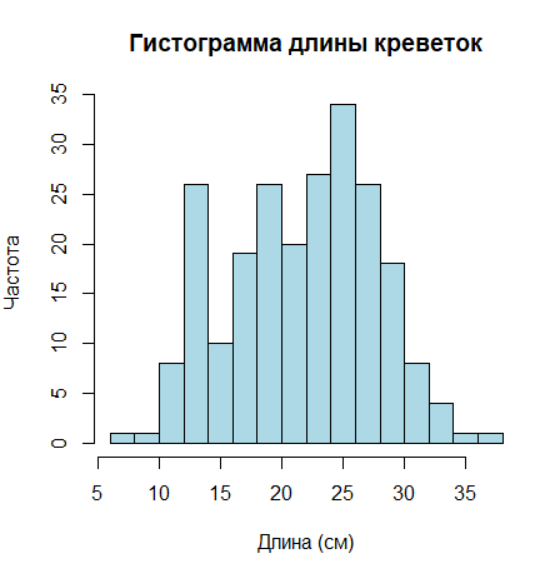
\includegraphics[width=0.6\linewidth,height=\textheight,keepaspectratio]{images/hist_shrimp.PNG}

}

\caption{Рис. 1.1: Гистограмма длины креветок}

\end{figure}%

\subsection{\texorpdfstring{Визуализация в
\texttt{ggridges}}{Визуализация в ggridges}}\label{ux432ux438ux437ux443ux430ux43bux438ux437ux430ux446ux438ux44f-ux432-ggridges}

Для элегантных и компактных графиков подходит библиотека
\texttt{ggridges}. Посторим распределение длины креветки в зависимости
от пола и возраста.

\begin{Shaded}
\begin{Highlighting}[]
\FunctionTok{library}\NormalTok{(ggplot2)}
\FunctionTok{library}\NormalTok{(ggridges)}

\FunctionTok{ggplot}\NormalTok{(data, }\FunctionTok{aes}\NormalTok{(}\AttributeTok{x =}\NormalTok{ length, }
                 \AttributeTok{y =}\NormalTok{ sex, }
                 \AttributeTok{group =}\NormalTok{ sex, }
                 \AttributeTok{fill =}\NormalTok{ sex)) }\SpecialCharTok{+}
  \FunctionTok{geom\_density\_ridges}\NormalTok{(}\AttributeTok{scale =} \DecValTok{2}\NormalTok{, }\AttributeTok{alpha =} \FloatTok{0.7}\NormalTok{) }\SpecialCharTok{+}
  \FunctionTok{scale\_y\_discrete}\NormalTok{(}\AttributeTok{expand =} \FunctionTok{c}\NormalTok{(}\DecValTok{0}\NormalTok{, }\DecValTok{0}\NormalTok{)) }\SpecialCharTok{+}
  \FunctionTok{scale\_x\_continuous}\NormalTok{(}\AttributeTok{expand =} \FunctionTok{c}\NormalTok{(}\DecValTok{0}\NormalTok{, }\DecValTok{0}\NormalTok{)) }\SpecialCharTok{+}
  \FunctionTok{labs}\NormalTok{(}
    \AttributeTok{title =} \StringTok{"Распределение длины карапакса по полу"}\NormalTok{,}
    \AttributeTok{x =} \StringTok{"Длина карапакса (мм)"}\NormalTok{,}
    \AttributeTok{y =} \StringTok{"Пол"}
\NormalTok{  ) }\SpecialCharTok{+}
  \FunctionTok{theme}\NormalTok{(}
    \AttributeTok{panel.border =} \FunctionTok{element\_blank}\NormalTok{(),  }\CommentTok{\# Убирает рамку вокруг графика}
    \AttributeTok{axis.line =} \FunctionTok{element\_line}\NormalTok{(}\AttributeTok{color =} \StringTok{"black"}\NormalTok{)  }\CommentTok{\# Сохраняет осевые линии (опционально)}
\NormalTok{  )}
\end{Highlighting}
\end{Shaded}

\begin{figure}[H]

{\centering 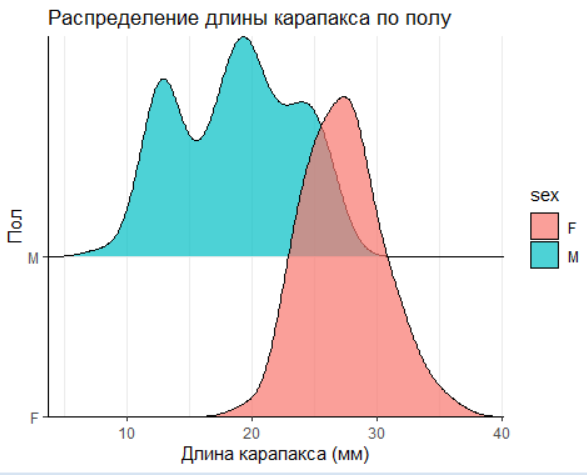
\includegraphics[width=0.6\linewidth,height=\textheight,keepaspectratio]{images/ggridges_shrimp.PNG}

}

\caption{Рис. 1.2: Пол-длина креветок с использованием
\texttt{ggridges}}

\end{figure}%

\section{Выявление аутлайеров
(выбросов)}\label{ux432ux44bux44fux432ux43bux435ux43dux438ux435-ux430ux443ux442ux43bux430ux439ux435ux440ux43eux432-ux432ux44bux431ux440ux43eux441ux43eux432}

Аутлаеры (выбросы) --- наблюдения, значительно отклоняющиеся от общего
распределения данных. Их идентификация критически важна, так как они
могут искажать результаты анализа. Один из надёжных методов обнаружения
выбросов --- \textbf{метод межквартильного размаха (IQR)}.

\subsection{\texorpdfstring{\textbf{Теория
метода}}{Теория метода}}\label{ux442ux435ux43eux440ux438ux44f-ux43cux435ux442ux43eux434ux430}

\begin{enumerate}
\def\labelenumi{\arabic{enumi}.}
\item
  \textbf{Расчёт квартилей}:

  \begin{itemize}
  \item
    \textbf{Q1} (25-й перцентиль): значение, ниже которого находится
    25\% данных.
  \item
    \textbf{Q3} (75-й перцентиль): значение, ниже которого находится
    75\% данных.
  \item
    \textbf{IQR = Q3 - Q1}: мера разброса средней половины данных.
  \end{itemize}
\item
  \textbf{Границы аутлаеров}:

  \begin{itemize}
  \item
    \textbf{Нижняя граница}: Q1−1.5×IQRQ1−1.5×IQR
  \item
    \textbf{Верхняя граница}: Q3+1.5×IQRQ3+1.5×IQR\\
    Наблюдения за этими пределами считаются выбросами.
  \end{itemize}
\end{enumerate}

\subsection{\texorpdfstring{\textbf{Преимущества
метода}}{Преимущества метода}}\label{ux43fux440ux435ux438ux43cux443ux449ux435ux441ux442ux432ux430-ux43cux435ux442ux43eux434ux430}

\begin{itemize}
\item
  Устойчивость к асимметрии распределения.
\item
  Не требует предположения о нормальности данных.
\end{itemize}

\begin{Shaded}
\begin{Highlighting}[]
\CommentTok{\# Метод межквартильного размаха}
\NormalTok{outliers }\OtherTok{\textless{}{-}}\NormalTok{ data }\SpecialCharTok{\%\textgreater{}\%}
  \FunctionTok{mutate}\NormalTok{(}
    \AttributeTok{length\_z =} \FunctionTok{scale}\NormalTok{(length),}
    \AttributeTok{weight\_z =} \FunctionTok{scale}\NormalTok{(weight)}
\NormalTok{  ) }\SpecialCharTok{\%\textgreater{}\%} 
  \FunctionTok{filter}\NormalTok{(}\FunctionTok{abs}\NormalTok{(length\_z) }\SpecialCharTok{\textgreater{}} \DecValTok{3} \SpecialCharTok{|} \FunctionTok{abs}\NormalTok{(weight\_z) }\SpecialCharTok{\textgreater{}} \DecValTok{3}\NormalTok{)}

\CommentTok{\# Визуализация}
\FunctionTok{ggplot}\NormalTok{(data, }\FunctionTok{aes}\NormalTok{(}\AttributeTok{x =}\NormalTok{ length, }\AttributeTok{y =}\NormalTok{ weight)) }\SpecialCharTok{+}
  \FunctionTok{geom\_point}\NormalTok{(}\FunctionTok{aes}\NormalTok{(}\AttributeTok{color =} \StringTok{"Обычные"}\NormalTok{), }\AttributeTok{alpha =} \FloatTok{0.5}\NormalTok{) }\SpecialCharTok{+}
  \FunctionTok{geom\_point}\NormalTok{(}\AttributeTok{data =}\NormalTok{ outliers, }\FunctionTok{aes}\NormalTok{(}\AttributeTok{color =} \StringTok{"Аутлаеры"}\NormalTok{), }\AttributeTok{size =} \DecValTok{3}\NormalTok{) }\SpecialCharTok{+}
  \FunctionTok{scale\_color\_manual}\NormalTok{(}\AttributeTok{values =} \FunctionTok{c}\NormalTok{(}\StringTok{"Обычные"} \OtherTok{=} \StringTok{"grey50"}\NormalTok{, }\StringTok{"Аутлаеры"} \OtherTok{=} \StringTok{"red"}\NormalTok{)) }\SpecialCharTok{+}
  \FunctionTok{labs}\NormalTok{(}\AttributeTok{title =} \StringTok{"Выявление аномальных наблюдений"}\NormalTok{, }\AttributeTok{color =} \StringTok{"Тип"}\NormalTok{)}
\end{Highlighting}
\end{Shaded}

\begin{figure}[H]

{\centering 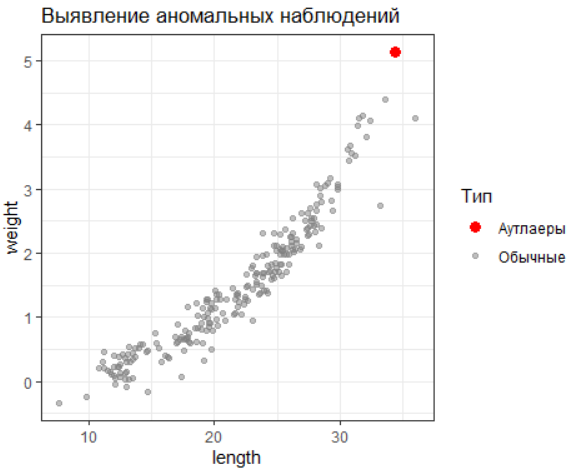
\includegraphics[width=0.6\linewidth,height=\textheight,keepaspectratio]{images/outliers_shrimp.PNG}

}

\caption{Рис. 1.3: Распределение длины карапакса}

\end{figure}%

\section{Определение возрастной структуры: статистические методы анализа
размерных
данных}\label{ux43eux43fux440ux435ux434ux435ux43bux435ux43dux438ux435-ux432ux43eux437ux440ux430ux441ux442ux43dux43eux439-ux441ux442ux440ux443ux43aux442ux443ux440ux44b-ux441ux442ux430ux442ux438ux441ux442ux438ux447ux435ux441ux43aux438ux435-ux43cux435ux442ux43eux434ux44b-ux430ux43dux430ux43bux438ux437ux430-ux440ux430ux437ux43cux435ux440ux43dux44bux445-ux434ux430ux43dux43dux44bux445}

Возрастная структура популяции --- часто важна для расчёта промысловой
смертности, оценки репродуктивного потенциала и прогнозирования динамики
запасов. Поскольку прямое измерение возраста часто невозможно (например,
у беспозвоночных или рыб без четких возрастных меток), используются
статистические методы, выделяющие группы в смешанных распределениях
размеров.

\textbf{Основные подходы:}

\begin{enumerate}
\def\labelenumi{\arabic{enumi}.}
\item
  \textbf{Метод k-средних (k-means)} --- алгоритм кластеризации,
  группирующий особи в заданное число кластеров (возрастных групп) на
  основе их размеров.
\item
  \textbf{Метод Бхаттачарии} --- статистический подход для разделения
  смешанных нормальных распределений, часто применяемый для
  идентификации мод в гистограммах.
\item
  \textbf{EM-алгоритм} --- оценка параметров смеси распределений,
  подходящая для данных с перекрывающимися возрастными группами.
\item
  \textbf{Гауссовы смеси (GMM)} --- расширение метода Бхаттачарии для
  многомерного анализа.
\item
  \textbf{Ядерное сглаживание} --- непараметрический метод визуализации
  плотности, помогающий выявить скрытые моды.
\end{enumerate}

Рассмотрим метод k-средних (k-means) и метод Бхаттачарии, предварительно
построив гистограмму.

\begin{Shaded}
\begin{Highlighting}[]
\CommentTok{\# Загрузка библиотек}
\FunctionTok{library}\NormalTok{(tidyverse)}
\FunctionTok{library}\NormalTok{(mixtools)}
\CommentTok{\# Гистограмма длины с наложением плотности}
\FunctionTok{ggplot}\NormalTok{(data, }\FunctionTok{aes}\NormalTok{(}\AttributeTok{x =}\NormalTok{ length)) }\SpecialCharTok{+}
  \FunctionTok{geom\_histogram}\NormalTok{(}\FunctionTok{aes}\NormalTok{(}\AttributeTok{y =} \FunctionTok{after\_stat}\NormalTok{(density)), }\AttributeTok{fill =} \StringTok{"steelblue"}\NormalTok{, }\AttributeTok{bins =} \DecValTok{20}\NormalTok{, }\AttributeTok{alpha =} \FloatTok{0.7}\NormalTok{) }\SpecialCharTok{+}
  \FunctionTok{geom\_density}\NormalTok{(}\AttributeTok{color =} \StringTok{"\#FC4E07"}\NormalTok{, }\AttributeTok{linewidth =} \DecValTok{1}\NormalTok{) }\SpecialCharTok{+}
  \FunctionTok{labs}\NormalTok{(}\AttributeTok{title =} \StringTok{"Распределение длины карапакса"}\NormalTok{, }
       \AttributeTok{subtitle =} \StringTok{"Пики могут соответствовать возрастным группам"}\NormalTok{,}
       \AttributeTok{x =} \StringTok{"Длина (мм)"}\NormalTok{)}
\end{Highlighting}
\end{Shaded}

\begin{figure}[H]

{\centering 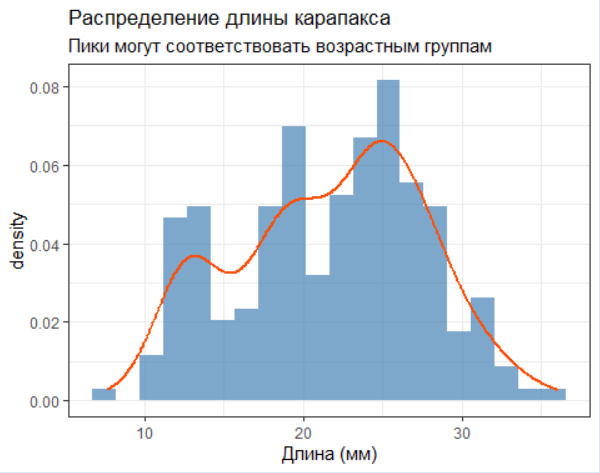
\includegraphics[width=0.6\linewidth,height=\textheight,keepaspectratio]{images/hist_dens_shrimp.PNG}

}

\caption{Рис. 1.3: Распределение длины карапакса}

\end{figure}%

\begin{Shaded}
\begin{Highlighting}[]
\CommentTok{\# Кластеризация по длине (K{-}means как пример)}
\FunctionTok{set.seed}\NormalTok{(}\DecValTok{123}\NormalTok{)}
\NormalTok{clusters }\OtherTok{\textless{}{-}} \FunctionTok{kmeans}\NormalTok{(data}\SpecialCharTok{$}\NormalTok{length, }\AttributeTok{centers =} \DecValTok{4}\NormalTok{)  }\CommentTok{\# Предполагаем 4 возрастные группы}
\NormalTok{data}\SpecialCharTok{$}\NormalTok{cluster }\OtherTok{\textless{}{-}} \FunctionTok{factor}\NormalTok{(clusters}\SpecialCharTok{$}\NormalTok{cluster)}

\CommentTok{\# Визуализация кластеров}
\FunctionTok{ggplot}\NormalTok{(data, }\FunctionTok{aes}\NormalTok{(}\AttributeTok{x =}\NormalTok{ length, }\AttributeTok{fill =}\NormalTok{ cluster)) }\SpecialCharTok{+}
  \FunctionTok{geom\_histogram}\NormalTok{(}\AttributeTok{bins =} \DecValTok{25}\NormalTok{, }\AttributeTok{alpha =} \FloatTok{0.7}\NormalTok{) }\SpecialCharTok{+}
  \FunctionTok{labs}\NormalTok{(}\AttributeTok{title =} \StringTok{"Кластеризация по длине)"}\NormalTok{, }
       \AttributeTok{x =} \StringTok{"Длина (мм)"}\NormalTok{)}
\end{Highlighting}
\end{Shaded}

\begin{figure}[H]

{\centering 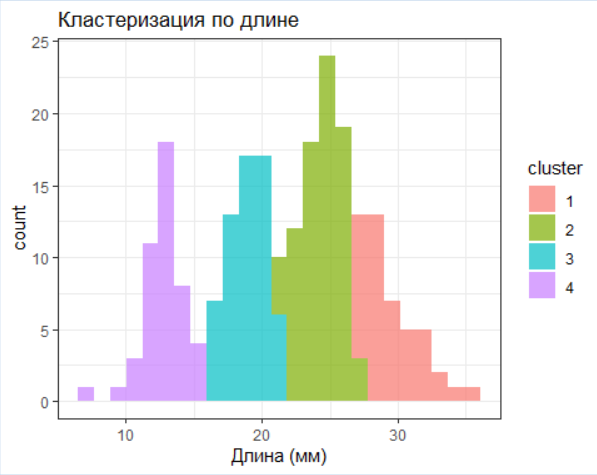
\includegraphics[width=0.6\linewidth,height=\textheight,keepaspectratio]{images/cluster_shrimp.PNG}

}

\caption{Рис. 1.4: Кластеризация по длине}

\end{figure}%

\begin{Shaded}
\begin{Highlighting}[]
\CommentTok{\# Установка рабочей директории}
\FunctionTok{setwd}\NormalTok{(}\StringTok{"C:/TEXTBOOK/"}\NormalTok{)}

\CommentTok{\# Загрузка библиотек}
\FunctionTok{library}\NormalTok{(tidyverse)}
\FunctionTok{library}\NormalTok{(mixtools)}

\CommentTok{\# Загрузка данных}
\NormalTok{data }\OtherTok{\textless{}{-}} \FunctionTok{read.csv}\NormalTok{(}\StringTok{"shrimp\_catch.csv"}\NormalTok{)}

\CommentTok{\# 1. Построение и отображение гистограммы}
\FunctionTok{hist}\NormalTok{(data}\SpecialCharTok{$}\NormalTok{length, }\AttributeTok{breaks =} \DecValTok{20}\NormalTok{, }\AttributeTok{main =} \StringTok{"Гистограмма распределения длин карапаксов"}\NormalTok{,}
     \AttributeTok{xlab =} \StringTok{"Длина карапакса (мм)"}\NormalTok{, }\AttributeTok{ylab =} \StringTok{"Частота"}\NormalTok{)}

\CommentTok{\# 2. Инициализация параметров (предположим 4 возрастные группы)}
\NormalTok{init\_params }\OtherTok{\textless{}{-}} \FunctionTok{list}\NormalTok{(}
  \AttributeTok{lambda =} \FunctionTok{rep}\NormalTok{(}\DecValTok{1}\SpecialCharTok{/}\DecValTok{4}\NormalTok{, }\DecValTok{4}\NormalTok{),}
  \AttributeTok{mu =} \FunctionTok{c}\NormalTok{(}\DecValTok{13}\NormalTok{, }\DecValTok{19}\NormalTok{, }\DecValTok{25}\NormalTok{, }\DecValTok{32}\NormalTok{),}
  \AttributeTok{sigma =} \FunctionTok{c}\NormalTok{(}\FloatTok{1.5}\NormalTok{, }\FloatTok{1.75}\NormalTok{, }\FloatTok{1.75}\NormalTok{, }\FloatTok{2.5}\NormalTok{)}
\NormalTok{)}

\CommentTok{\# 3. Разделение смеси распределений методом EM}
\NormalTok{fit }\OtherTok{\textless{}{-}} \FunctionTok{normalmixEM}\NormalTok{(data}\SpecialCharTok{$}\NormalTok{length, }\AttributeTok{k =} \DecValTok{4}\NormalTok{, }\AttributeTok{maxit =} \DecValTok{1000}\NormalTok{, }\AttributeTok{epsilon =} \FloatTok{1e{-}3}\NormalTok{,}
                   \AttributeTok{lambda =}\NormalTok{ init\_params}\SpecialCharTok{$}\NormalTok{lambda,}
                   \AttributeTok{mu =}\NormalTok{ init\_params}\SpecialCharTok{$}\NormalTok{mu,}
                   \AttributeTok{sigma =}\NormalTok{ init\_params}\SpecialCharTok{$}\NormalTok{sigma)}

\CommentTok{\# 4. Визуализация результатов с ggplot2}
\CommentTok{\# Генерация сетки для построения кривых}
\NormalTok{x\_grid }\OtherTok{\textless{}{-}} \FunctionTok{seq}\NormalTok{(}\FunctionTok{min}\NormalTok{(data}\SpecialCharTok{$}\NormalTok{length), }\FunctionTok{max}\NormalTok{(data}\SpecialCharTok{$}\NormalTok{length), }\AttributeTok{length.out =} \DecValTok{500}\NormalTok{)}

\CommentTok{\# Функция смеси}
\NormalTok{mixture\_density }\OtherTok{\textless{}{-}} \ControlFlowTok{function}\NormalTok{(x) \{}
\NormalTok{  fit}\SpecialCharTok{$}\NormalTok{lambda[}\DecValTok{1}\NormalTok{] }\SpecialCharTok{*} \FunctionTok{dnorm}\NormalTok{(x, fit}\SpecialCharTok{$}\NormalTok{mu[}\DecValTok{1}\NormalTok{], fit}\SpecialCharTok{$}\NormalTok{sigma[}\DecValTok{1}\NormalTok{]) }\SpecialCharTok{+}
\NormalTok{  fit}\SpecialCharTok{$}\NormalTok{lambda[}\DecValTok{2}\NormalTok{] }\SpecialCharTok{*} \FunctionTok{dnorm}\NormalTok{(x, fit}\SpecialCharTok{$}\NormalTok{mu[}\DecValTok{2}\NormalTok{], fit}\SpecialCharTok{$}\NormalTok{sigma[}\DecValTok{2}\NormalTok{]) }\SpecialCharTok{+}
\NormalTok{  fit}\SpecialCharTok{$}\NormalTok{lambda[}\DecValTok{3}\NormalTok{] }\SpecialCharTok{*} \FunctionTok{dnorm}\NormalTok{(x, fit}\SpecialCharTok{$}\NormalTok{mu[}\DecValTok{3}\NormalTok{], fit}\SpecialCharTok{$}\NormalTok{sigma[}\DecValTok{3}\NormalTok{]) }\SpecialCharTok{+}
\NormalTok{  fit}\SpecialCharTok{$}\NormalTok{lambda[}\DecValTok{4}\NormalTok{] }\SpecialCharTok{*} \FunctionTok{dnorm}\NormalTok{(x, fit}\SpecialCharTok{$}\NormalTok{mu[}\DecValTok{4}\NormalTok{], fit}\SpecialCharTok{$}\NormalTok{sigma[}\DecValTok{4}\NormalTok{])}
\NormalTok{\}}

\CommentTok{\# График}
\FunctionTok{ggplot}\NormalTok{(data, }\FunctionTok{aes}\NormalTok{(}\AttributeTok{x =}\NormalTok{ length)) }\SpecialCharTok{+}
  \CommentTok{\# Гистограмма}
  \FunctionTok{geom\_histogram}\NormalTok{(}\FunctionTok{aes}\NormalTok{(}\AttributeTok{y =} \FunctionTok{after\_stat}\NormalTok{(density)), }\AttributeTok{bins =} \DecValTok{20}\NormalTok{, }\AttributeTok{fill =} \StringTok{"white"}\NormalTok{, }\AttributeTok{color =} \StringTok{"black"}\NormalTok{, }\AttributeTok{alpha =} \FloatTok{0.7}\NormalTok{) }\SpecialCharTok{+}
  \CommentTok{\# Исходное распределение (гладкая линия)}
  \FunctionTok{geom\_density}\NormalTok{(}\AttributeTok{color =} \StringTok{"red"}\NormalTok{, }\AttributeTok{lwd =} \FloatTok{1.2}\NormalTok{) }\SpecialCharTok{+}
  \CommentTok{\# Смесь распределений}
  \FunctionTok{stat\_function}\NormalTok{(}\AttributeTok{fun =}\NormalTok{ mixture\_density, }\AttributeTok{color =} \StringTok{"black"}\NormalTok{, }\AttributeTok{lwd =} \FloatTok{1.5}\NormalTok{) }\SpecialCharTok{+}
  \CommentTok{\# Компоненты смеси}
  \FunctionTok{stat\_function}\NormalTok{(}\AttributeTok{fun =} \ControlFlowTok{function}\NormalTok{(x) fit}\SpecialCharTok{$}\NormalTok{lambda[}\DecValTok{1}\NormalTok{] }\SpecialCharTok{*} \FunctionTok{dnorm}\NormalTok{(x, fit}\SpecialCharTok{$}\NormalTok{mu[}\DecValTok{1}\NormalTok{], fit}\SpecialCharTok{$}\NormalTok{sigma[}\DecValTok{1}\NormalTok{]), }\AttributeTok{color =} \StringTok{"blue"}\NormalTok{, }\AttributeTok{lwd =} \DecValTok{1}\NormalTok{) }\SpecialCharTok{+}
  \FunctionTok{stat\_function}\NormalTok{(}\AttributeTok{fun =} \ControlFlowTok{function}\NormalTok{(x) fit}\SpecialCharTok{$}\NormalTok{lambda[}\DecValTok{2}\NormalTok{] }\SpecialCharTok{*} \FunctionTok{dnorm}\NormalTok{(x, fit}\SpecialCharTok{$}\NormalTok{mu[}\DecValTok{2}\NormalTok{], fit}\SpecialCharTok{$}\NormalTok{sigma[}\DecValTok{2}\NormalTok{]), }\AttributeTok{color =} \StringTok{"green"}\NormalTok{, }\AttributeTok{lwd =} \DecValTok{1}\NormalTok{) }\SpecialCharTok{+}
  \FunctionTok{stat\_function}\NormalTok{(}\AttributeTok{fun =} \ControlFlowTok{function}\NormalTok{(x) fit}\SpecialCharTok{$}\NormalTok{lambda[}\DecValTok{3}\NormalTok{] }\SpecialCharTok{*} \FunctionTok{dnorm}\NormalTok{(x, fit}\SpecialCharTok{$}\NormalTok{mu[}\DecValTok{3}\NormalTok{], fit}\SpecialCharTok{$}\NormalTok{sigma[}\DecValTok{3}\NormalTok{]), }\AttributeTok{color =} \StringTok{"orange"}\NormalTok{, }\AttributeTok{lwd =} \DecValTok{1}\NormalTok{) }\SpecialCharTok{+}
  \FunctionTok{stat\_function}\NormalTok{(}\AttributeTok{fun =} \ControlFlowTok{function}\NormalTok{(x) fit}\SpecialCharTok{$}\NormalTok{lambda[}\DecValTok{4}\NormalTok{] }\SpecialCharTok{*} \FunctionTok{dnorm}\NormalTok{(x, fit}\SpecialCharTok{$}\NormalTok{mu[}\DecValTok{4}\NormalTok{], fit}\SpecialCharTok{$}\NormalTok{sigma[}\DecValTok{4}\NormalTok{]), }\AttributeTok{color =} \StringTok{"purple"}\NormalTok{, }\AttributeTok{lwd =} \DecValTok{1}\NormalTok{) }\SpecialCharTok{+}
  
  \CommentTok{\# Настройка темы и легенды}
  \FunctionTok{theme\_minimal}\NormalTok{() }\SpecialCharTok{+}
  \FunctionTok{labs}\NormalTok{(}
    \AttributeTok{x =} \StringTok{"Длина карапакса (мм)"}\NormalTok{,}
    \AttributeTok{y =} \StringTok{"Плотность"}\NormalTok{,}
    \AttributeTok{title =} \StringTok{"Разделение возрастных групп методом EM"}
\NormalTok{  )}
\end{Highlighting}
\end{Shaded}

\begin{figure}[H]

{\centering 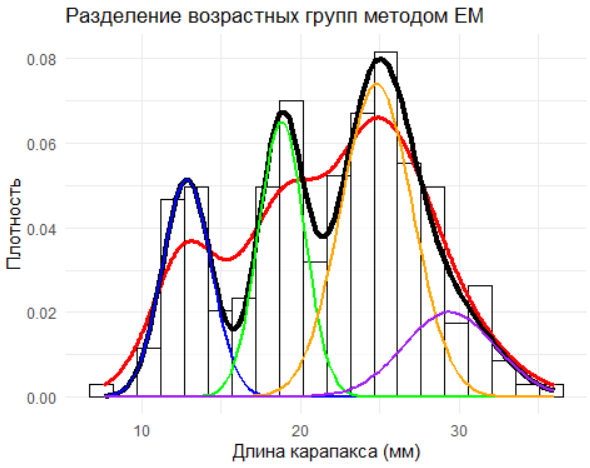
\includegraphics[width=0.6\linewidth,height=\textheight,keepaspectratio]{images/bhattacharya_shrimp.PNG}

}

\caption{Рис. 1.5: Метод Бхаттачарии}

\end{figure}%

\section{Уравнение
Берталанфи}\label{ux443ux440ux430ux432ux43dux435ux43dux438ux435-ux431ux435ux440ux442ux430ux43bux430ux43dux444ux438}

Уравнение Берталанфи --- фундаментальная модель в рыбохозяйственной
науке, описывающая асимптотический рост организмов. Оно имеет вид: \[
L(t) = L_{\infty} \cdot \left(1 - e^{-k \cdot (t - t_0)}\right)
\] где \emph{L\textsubscript{∞}}--- теоретическая максимальная длина
особи, \emph{k}--- коэффициент скорости роста,
\emph{t\textsubscript{0}}--- гипотетический возраст при нулевой длине.

В приведённом коде модель применяется для анализа роста северной
креветки :

\begin{enumerate}
\def\labelenumi{\arabic{enumi}.}
\item
  \textbf{Подготовка данных}: Удаление аутлаеров (например, строк 10 и
  50) повышает точность оценки параметров.
\item
  \textbf{Инициализация параметров}:

  \begin{itemize}
  \item
    \emph{L\textsubscript{∞}} задаётся как максимальная наблюдаемая
    длина в данных.
  \item
    \emph{k} и \emph{t\textsubscript{0}} подбираются итеративно методом
    нелинейных наименьших квадратов (\textbf{\texttt{nls}}).
  \end{itemize}
\item
  \textbf{Визуализация}: График сопоставляет эмпирические данные (точки)
  с предсказаниями модели (красная линия), демонстрируя, как рост
  замедляется с приближением к \emph{L∞}.
\end{enumerate}

\textbf{Интерпретация параметров}:

\begin{itemize}
\item
  Высокое значение \emph{k} (\textgreater0.3) указывает на быстрый рост
  молоди.
\item
  \emph{t\textsubscript{0}}\textless0 может отражать ранний метаморфоз
  личинок.
\end{itemize}

\begin{Shaded}
\begin{Highlighting}[]
\CommentTok{\# Загрузка библиотек}
\FunctionTok{library}\NormalTok{(ggplot2)}
\FunctionTok{library}\NormalTok{(dplyr)}
\FunctionTok{library}\NormalTok{(nlme)}

\CommentTok{\# Загрузка данных}
\NormalTok{data }\OtherTok{\textless{}{-}} \FunctionTok{read.csv}\NormalTok{(}\StringTok{"shrimp\_catch.csv"}\NormalTok{)}

\CommentTok{\# Преобразование возраста в числовой формат}
\NormalTok{data}\SpecialCharTok{$}\NormalTok{age\_num }\OtherTok{\textless{}{-}} \FunctionTok{as.numeric}\NormalTok{(data}\SpecialCharTok{$}\NormalTok{age)}

\CommentTok{\# Удаление аутлайеров (если необходимо)}
\NormalTok{data\_clean }\OtherTok{\textless{}{-}}\NormalTok{ data }\SpecialCharTok{\%\textgreater{}\%}
  \FunctionTok{filter}\NormalTok{(}\SpecialCharTok{!}\NormalTok{id }\SpecialCharTok{\%in\%} \FunctionTok{c}\NormalTok{(}\DecValTok{10}\NormalTok{, }\DecValTok{50}\NormalTok{))  }\CommentTok{\# Пример удаления строк с аномалиями}

\CommentTok{\# Начальные параметры на основе данных}
\NormalTok{L\_inf\_start }\OtherTok{\textless{}{-}} \FunctionTok{max}\NormalTok{(data\_clean}\SpecialCharTok{$}\NormalTok{length, }\AttributeTok{na.rm =} \ConstantTok{TRUE}\NormalTok{)  }\CommentTok{\# Максимальная длина}
\NormalTok{k\_start }\OtherTok{\textless{}{-}} \FloatTok{0.3}                                        \CommentTok{\# Средняя скорость роста}
\NormalTok{t0\_start }\OtherTok{\textless{}{-}} \SpecialCharTok{{-}}\FloatTok{0.5}                                      \CommentTok{\# Гипотетический возраст}

\CommentTok{\# Подгонка модели с увеличенным числом итераций}
\NormalTok{model }\OtherTok{\textless{}{-}} \FunctionTok{nls}\NormalTok{(}
\NormalTok{  length }\SpecialCharTok{\textasciitilde{}}\NormalTok{ L\_inf }\SpecialCharTok{*}\NormalTok{ (}\DecValTok{1} \SpecialCharTok{{-}} \FunctionTok{exp}\NormalTok{(}\SpecialCharTok{{-}}\NormalTok{k }\SpecialCharTok{*}\NormalTok{ (age\_num }\SpecialCharTok{{-}}\NormalTok{ t0))),}
  \AttributeTok{data =}\NormalTok{ data\_clean,}
  \AttributeTok{start =} \FunctionTok{list}\NormalTok{(}\AttributeTok{L\_inf =}\NormalTok{ L\_inf\_start, }\AttributeTok{k =}\NormalTok{ k\_start, }\AttributeTok{t0 =}\NormalTok{ t0\_start),}
  \AttributeTok{control =} \FunctionTok{nls.control}\NormalTok{(}\AttributeTok{maxiter =} \DecValTok{200}\NormalTok{, }\AttributeTok{warnOnly =} \ConstantTok{TRUE}\NormalTok{)  }\CommentTok{\# Увеличиваем лимит итераций}
\NormalTok{)}

\CommentTok{\# Вывод результатов}
\FunctionTok{summary}\NormalTok{(model)}

\CommentTok{\# Создание последовательности возрастов для предсказания}
\NormalTok{age\_seq }\OtherTok{\textless{}{-}} \FunctionTok{seq}\NormalTok{(}\FunctionTok{min}\NormalTok{(data\_clean}\SpecialCharTok{$}\NormalTok{age\_num), }\FunctionTok{max}\NormalTok{(data\_clean}\SpecialCharTok{$}\NormalTok{age\_num), }\AttributeTok{by =} \FloatTok{0.1}\NormalTok{)}

\CommentTok{\# Предсказание значений длины}
\NormalTok{length\_pred }\OtherTok{\textless{}{-}} \FunctionTok{predict}\NormalTok{(model, }\AttributeTok{newdata =} \FunctionTok{data.frame}\NormalTok{(}\AttributeTok{age\_num =}\NormalTok{ age\_seq))}

\CommentTok{\# Построение графика}
\FunctionTok{ggplot}\NormalTok{(data\_clean, }\FunctionTok{aes}\NormalTok{(}\AttributeTok{x =}\NormalTok{ age\_num, }\AttributeTok{y =}\NormalTok{ length)) }\SpecialCharTok{+}
  \FunctionTok{geom\_point}\NormalTok{(}\FunctionTok{aes}\NormalTok{(}\AttributeTok{color =}\NormalTok{ age), }\AttributeTok{alpha =} \FloatTok{0.7}\NormalTok{) }\SpecialCharTok{+}
  \FunctionTok{geom\_line}\NormalTok{(}\AttributeTok{data =} \FunctionTok{data.frame}\NormalTok{(}\AttributeTok{age\_num =}\NormalTok{ age\_seq, }\AttributeTok{length =}\NormalTok{ length\_pred), }
            \FunctionTok{aes}\NormalTok{(}\AttributeTok{x =}\NormalTok{ age\_num, }\AttributeTok{y =}\NormalTok{ length), }\AttributeTok{color =} \StringTok{"red"}\NormalTok{, }\AttributeTok{linewidth =} \FloatTok{1.2}\NormalTok{) }\SpecialCharTok{+}
  \FunctionTok{labs}\NormalTok{(}
    \AttributeTok{title =} \StringTok{"Рост креветок по уравнению Берталанфи"}\NormalTok{,}
    \AttributeTok{x =} \StringTok{"Возраст (годы)"}\NormalTok{,}
    \AttributeTok{y =} \StringTok{"Длина карапакса (мм)"}\NormalTok{,}
    \AttributeTok{color =} \StringTok{"Возрастная группа"}
\NormalTok{  ) }\SpecialCharTok{+}
  \FunctionTok{theme\_minimal}\NormalTok{()}

\CommentTok{\# Сохранение графика}
\FunctionTok{ggsave}\NormalTok{(}\StringTok{"bertalanffy\_model.png"}\NormalTok{, }\AttributeTok{width =} \DecValTok{8}\NormalTok{, }\AttributeTok{height =} \DecValTok{6}\NormalTok{)}
\end{Highlighting}
\end{Shaded}

\begin{figure}[H]

{\centering 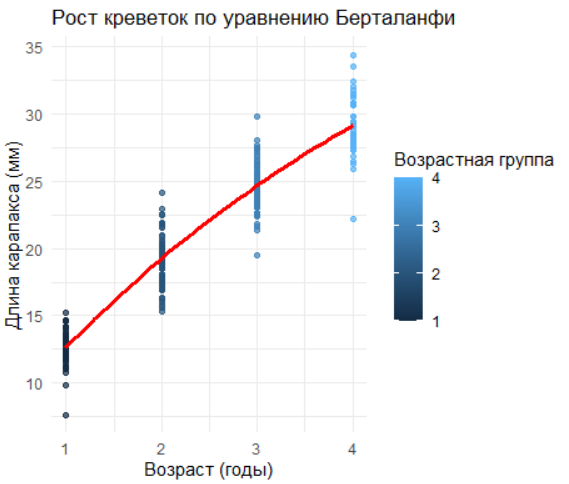
\includegraphics[width=0.6\linewidth,height=\textheight,keepaspectratio]{images/bertalanffy_model.PNG}

}

\caption{Рис. 1.6: Рост креветок по уравнению Берталанфи}

\end{figure}%

\section{Огива, логистическая кривая и 50\%-ное
созревание}\label{ux43eux433ux438ux432ux430-ux43bux43eux433ux438ux441ux442ux438ux447ux435ux441ux43aux430ux44f-ux43aux440ux438ux432ux430ux44f-ux438-50-ux43dux43eux435-ux441ux43eux437ux440ux435ux432ux430ux43dux438ux435}

Логистическая кривая --- ключевой инструмент для моделирования бинарных
процессов, таких как созревание или смена пола у организмов. В случае
протоандрических креветок (\emph{Pandalus borealis}), которые меняют пол
с возрастом, зависимость вероятности быть самкой от длины карапакса
можно описать логистической функцией:

\[
P(F) = \frac{1}{1 + e^{-(\beta_0 + \beta_1 \cdot длина)}}
\]

где \emph{P(F)} --- вероятность принадлежности к женскому полу,
\emph{β\textsubscript{0}} --- интерсепт, \emph{β\textsubscript{1}} ---
коэффициент влияния длины.

Точка перегиба логистической кривой соответствует длине, при которой
вероятность быть самкой равна 50\%: \[
L_{50} = -\frac{\beta_0}{\beta_1}
\]

\begin{figure}[H]

{\centering 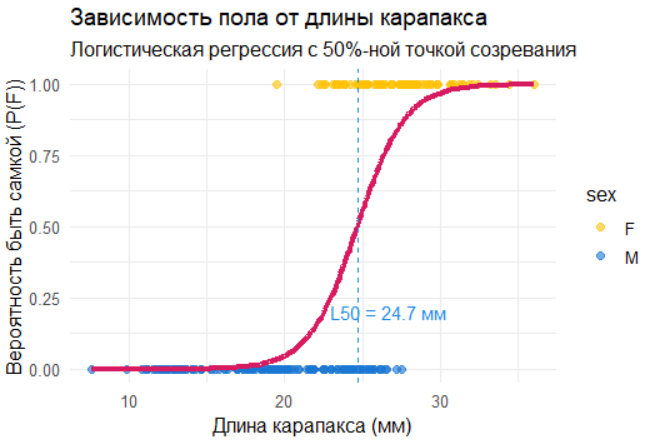
\includegraphics[width=0.6\linewidth,height=\textheight,keepaspectratio]{images/logistic_model_shrimp.PNG}

}

\caption{Рис. 1.7: Логистическая кривая}

\end{figure}%

Огива (кумулятивная кривая) показывает накопление вероятности с
увеличением длины. Для анализа созревания её можно построить через
интеграл логистической функции. Визуально она демонстрирует, как доля
самок возрастает с размером.

\begin{figure}[H]

{\centering 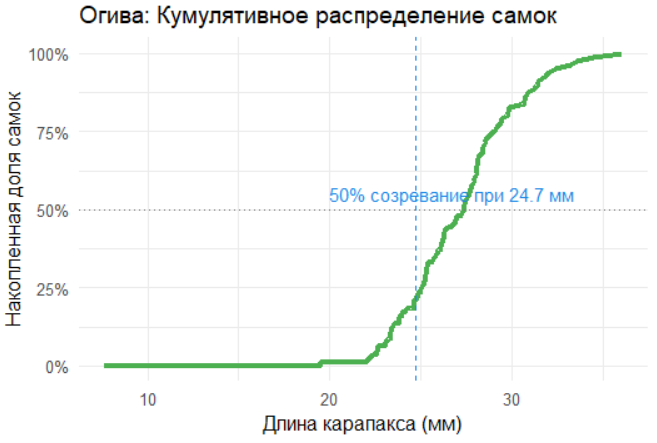
\includegraphics[width=0.6\linewidth,height=\textheight,keepaspectratio]{images/ogive_shrimp.PNG}

}

\caption{Рис. 1.8: Огива}

\end{figure}%

\subsection{\texorpdfstring{\textbf{Оценка
модели}}{Оценка модели}}\label{ux43eux446ux435ux43dux43aux430-ux43cux43eux434ux435ux43bux438}

\begin{enumerate}
\def\labelenumi{\arabic{enumi}.}
\item
  \textbf{ROC-кривая и AUC}:

  \begin{itemize}
  \item
    Площадь под ROC-кривой (AUC) \textgreater0.7 указывает на хорошую
    предсказательную способность модели.
  \item
    Значение AUC = 0.94(пример из кода) подтверждает сильную связь длины
    и пола.
  \end{itemize}
\end{enumerate}

\begin{figure}[H]

{\centering 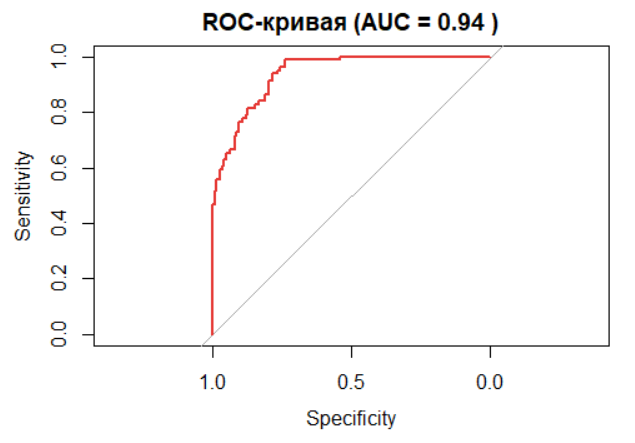
\includegraphics[width=0.6\linewidth,height=\textheight,keepaspectratio]{images/ROC_shrimp.PNG}

}

\caption{Рис. 1.9: ROC-кривая и AUC}

\end{figure}%

\begin{enumerate}
\def\labelenumi{\arabic{enumi}.}
\setcounter{enumi}{1}
\item
  \textbf{Интерпретация коэффициентов}:

  \begin{itemize}
  \item
    Положительный \emph{β\textsubscript{1}} означает: с ростом длины
    вероятность быть самкой увеличивается.
  \item
    Например, \emph{β\textsubscript{1}}=0.25 → увеличение длины на 1 мм
    повышает шансы в e\textsuperscript{0.25}≈1.28 раза.
  \end{itemize}
\end{enumerate}

\subsection{\texorpdfstring{\textbf{Биологический
контекст}}{Биологический контекст}}\label{ux431ux438ux43eux43bux43eux433ux438ux447ux435ux441ux43aux438ux439-ux43aux43eux43dux442ux435ux43aux441ux442}

\begin{itemize}
\item
  \textbf{Протоандрический гермафродитизм}: У креветок смена пола с
  самцов на самок происходит при достижении критического размера
  (\textasciitilde25-28 мм).
\item
  \textbf{L50 как индикатор}: Снижение \emph{L\textsubscript{50}} в
  популяции может сигнализировать о стрессовых условиях (перелов,
  изменение среды), ускоряющих созревание.
\end{itemize}

\begin{Shaded}
\begin{Highlighting}[]
\CommentTok{\# Установка рабочей директории}
\FunctionTok{setwd}\NormalTok{(}\StringTok{"C:/TEXTBOOK/"}\NormalTok{)}

\CommentTok{\# Загрузка библиотек}
\FunctionTok{library}\NormalTok{(tidyverse)}
\FunctionTok{library}\NormalTok{(pROC)}
\FunctionTok{library}\NormalTok{(ggplot2)}

\CommentTok{\# Загрузка данных}
\NormalTok{data }\OtherTok{\textless{}{-}} \FunctionTok{read\_csv}\NormalTok{(}\StringTok{"shrimp\_catch.csv"}\NormalTok{)}

\CommentTok{\# 1. Предобработка данных {-}{-}{-}{-}{-}{-}{-}{-}{-}{-}{-}{-}{-}{-}{-}{-}{-}{-}{-}{-}{-}{-}{-}{-}{-}{-}{-}{-}{-}{-}{-}{-}{-}{-}{-}{-}{-}{-}{-}{-}{-}{-}{-}{-}{-}{-}{-}{-}{-}{-}{-}{-}{-}}
\CommentTok{\# Удаление аутлаеров методом IQR}
\NormalTok{Q1 }\OtherTok{\textless{}{-}} \FunctionTok{quantile}\NormalTok{(data}\SpecialCharTok{$}\NormalTok{length, }\FloatTok{0.25}\NormalTok{)}
\NormalTok{Q3 }\OtherTok{\textless{}{-}} \FunctionTok{quantile}\NormalTok{(data}\SpecialCharTok{$}\NormalTok{length, }\FloatTok{0.75}\NormalTok{)}
\NormalTok{IQR }\OtherTok{\textless{}{-}}\NormalTok{ Q3 }\SpecialCharTok{{-}}\NormalTok{ Q1}
\NormalTok{data\_clean }\OtherTok{\textless{}{-}}\NormalTok{ data }\SpecialCharTok{\%\textgreater{}\%}
  \FunctionTok{filter}\NormalTok{(length }\SpecialCharTok{\textgreater{}=}\NormalTok{ Q1 }\SpecialCharTok{{-}} \FloatTok{1.5}\SpecialCharTok{*}\NormalTok{IQR }\SpecialCharTok{\&}\NormalTok{ length }\SpecialCharTok{\textless{}=}\NormalTok{ Q3 }\SpecialCharTok{+} \FloatTok{1.5}\SpecialCharTok{*}\NormalTok{IQR)}

\CommentTok{\# 2. Логистическая регрессия {-}{-}{-}{-}{-}{-}{-}{-}{-}{-}{-}{-}{-}{-}{-}{-}{-}{-}{-}{-}{-}{-}{-}{-}{-}{-}{-}{-}{-}{-}{-}{-}{-}{-}{-}{-}{-}{-}{-}{-}{-}{-}{-}{-}{-}{-}{-}{-}{-}{-}}
\CommentTok{\# Преобразование пола в бинарную переменную}
\NormalTok{data\_clean}\SpecialCharTok{$}\NormalTok{sex\_binary }\OtherTok{\textless{}{-}} \FunctionTok{ifelse}\NormalTok{(data\_clean}\SpecialCharTok{$}\NormalTok{sex }\SpecialCharTok{==} \StringTok{"F"}\NormalTok{, }\DecValTok{1}\NormalTok{, }\DecValTok{0}\NormalTok{)}

\CommentTok{\# Подгонка модели}
\NormalTok{model\_logit }\OtherTok{\textless{}{-}} \FunctionTok{glm}\NormalTok{(sex\_binary }\SpecialCharTok{\textasciitilde{}}\NormalTok{ length, }
                   \AttributeTok{data =}\NormalTok{ data\_clean, }
                   \AttributeTok{family =} \FunctionTok{binomial}\NormalTok{(}\AttributeTok{link =} \StringTok{"logit"}\NormalTok{))}

\CommentTok{\# Расчет коэффициентов}
\NormalTok{beta0 }\OtherTok{\textless{}{-}} \FunctionTok{coef}\NormalTok{(model\_logit)[}\DecValTok{1}\NormalTok{]}
\NormalTok{beta1 }\OtherTok{\textless{}{-}} \FunctionTok{coef}\NormalTok{(model\_logit)[}\DecValTok{2}\NormalTok{]}

\CommentTok{\# Вычисление L50 (длина 50\% созревания)}
\NormalTok{L50 }\OtherTok{\textless{}{-}} \FunctionTok{round}\NormalTok{(}\SpecialCharTok{{-}}\NormalTok{beta0}\SpecialCharTok{/}\NormalTok{beta1, }\DecValTok{1}\NormalTok{)}

\CommentTok{\# 3. Визуализация {-}{-}{-}{-}{-}{-}{-}{-}{-}{-}{-}{-}{-}{-}{-}{-}{-}{-}{-}{-}{-}{-}{-}{-}{-}{-}{-}{-}{-}{-}{-}{-}{-}{-}{-}{-}{-}{-}{-}{-}{-}{-}{-}{-}{-}{-}{-}{-}{-}{-}{-}{-}{-}{-}{-}{-}{-}{-}{-}{-}}
\CommentTok{\# Логистическая кривая}
\FunctionTok{ggplot}\NormalTok{(data\_clean, }\FunctionTok{aes}\NormalTok{(}\AttributeTok{x =}\NormalTok{ length, }\AttributeTok{y =}\NormalTok{ sex\_binary)) }\SpecialCharTok{+}
  \FunctionTok{geom\_point}\NormalTok{(}\FunctionTok{aes}\NormalTok{(}\AttributeTok{color =}\NormalTok{ sex), }\AttributeTok{alpha =} \FloatTok{0.6}\NormalTok{, }\AttributeTok{size =} \DecValTok{2}\NormalTok{) }\SpecialCharTok{+}
  \FunctionTok{geom\_line}\NormalTok{(}\FunctionTok{aes}\NormalTok{(}\AttributeTok{y =} \FunctionTok{predict}\NormalTok{(model\_logit, }\AttributeTok{type =} \StringTok{"response"}\NormalTok{)), }
            \AttributeTok{color =} \StringTok{"\#D81B60"}\NormalTok{, }\AttributeTok{linewidth =} \FloatTok{1.5}\NormalTok{) }\SpecialCharTok{+}
  \FunctionTok{geom\_vline}\NormalTok{(}\AttributeTok{xintercept =}\NormalTok{ L50, }\AttributeTok{linetype =} \StringTok{"dashed"}\NormalTok{, }\AttributeTok{color =} \StringTok{"\#1E88E5"}\NormalTok{) }\SpecialCharTok{+}
  \FunctionTok{annotate}\NormalTok{(}\StringTok{"text"}\NormalTok{, }\AttributeTok{x =}\NormalTok{ L50 }\SpecialCharTok{+} \DecValTok{2}\NormalTok{, }\AttributeTok{y =} \FloatTok{0.2}\NormalTok{, }
           \AttributeTok{label =} \FunctionTok{paste}\NormalTok{(}\StringTok{"L50 ="}\NormalTok{, L50, }\StringTok{"мм"}\NormalTok{), }\AttributeTok{color =} \StringTok{"\#1E88E5"}\NormalTok{) }\SpecialCharTok{+}
  \FunctionTok{scale\_color\_manual}\NormalTok{(}\AttributeTok{values =} \FunctionTok{c}\NormalTok{(}\StringTok{"\#FFC107"}\NormalTok{, }\StringTok{"\#1976D2"}\NormalTok{)) }\SpecialCharTok{+}
  \FunctionTok{labs}\NormalTok{(}
    \AttributeTok{title =} \StringTok{"Зависимость пола от длины карапакса"}\NormalTok{,}
    \AttributeTok{subtitle =} \StringTok{"Логистическая регрессия с 50\%{-}ной точкой созревания"}\NormalTok{,}
    \AttributeTok{x =} \StringTok{"Длина карапакса (мм)"}\NormalTok{,}
    \AttributeTok{y =} \StringTok{"Вероятность быть самкой (P(F))"}
\NormalTok{  ) }\SpecialCharTok{+}
  \FunctionTok{theme\_minimal}\NormalTok{(}\AttributeTok{base\_size =} \DecValTok{12}\NormalTok{)}

\CommentTok{\# Огива (кумулятивное распределение)}
\NormalTok{data\_ogive }\OtherTok{\textless{}{-}}\NormalTok{ data\_clean }\SpecialCharTok{\%\textgreater{}\%}
  \FunctionTok{arrange}\NormalTok{(length) }\SpecialCharTok{\%\textgreater{}\%}
  \FunctionTok{mutate}\NormalTok{(}
    \AttributeTok{cum\_females =} \FunctionTok{cumsum}\NormalTok{(sex\_binary),}
    \AttributeTok{cum\_prob =}\NormalTok{ cum\_females }\SpecialCharTok{/} \FunctionTok{max}\NormalTok{(cum\_females)}
\NormalTok{  )}

\FunctionTok{ggplot}\NormalTok{(data\_ogive, }\FunctionTok{aes}\NormalTok{(}\AttributeTok{x =}\NormalTok{ length, }\AttributeTok{y =}\NormalTok{ cum\_prob)) }\SpecialCharTok{+}
  \FunctionTok{geom\_line}\NormalTok{(}\AttributeTok{color =} \StringTok{"\#4CAF50"}\NormalTok{, }\AttributeTok{linewidth =} \FloatTok{1.5}\NormalTok{) }\SpecialCharTok{+}
  \FunctionTok{geom\_vline}\NormalTok{(}\AttributeTok{xintercept =}\NormalTok{ L50, }\AttributeTok{linetype =} \StringTok{"dashed"}\NormalTok{, }\AttributeTok{color =} \StringTok{"\#1E88E5"}\NormalTok{) }\SpecialCharTok{+}
  \FunctionTok{geom\_hline}\NormalTok{(}\AttributeTok{yintercept =} \FloatTok{0.5}\NormalTok{, }\AttributeTok{linetype =} \StringTok{"dotted"}\NormalTok{, }\AttributeTok{color =} \StringTok{"\#757575"}\NormalTok{) }\SpecialCharTok{+}
  \FunctionTok{annotate}\NormalTok{(}\StringTok{"text"}\NormalTok{, }\AttributeTok{x =}\NormalTok{ L50 }\SpecialCharTok{+} \DecValTok{2}\NormalTok{, }\AttributeTok{y =} \FloatTok{0.55}\NormalTok{, }
           \AttributeTok{label =} \FunctionTok{paste}\NormalTok{(}\StringTok{"50\% созревание при"}\NormalTok{, L50, }\StringTok{"мм"}\NormalTok{), }\AttributeTok{color =} \StringTok{"\#1E88E5"}\NormalTok{) }\SpecialCharTok{+}
  \FunctionTok{scale\_y\_continuous}\NormalTok{(}\AttributeTok{labels =}\NormalTok{ scales}\SpecialCharTok{::}\NormalTok{percent) }\SpecialCharTok{+}
  \FunctionTok{labs}\NormalTok{(}
    \AttributeTok{title =} \StringTok{"Огива: Кумулятивное распределение самок"}\NormalTok{,}
    \AttributeTok{x =} \StringTok{"Длина карапакса (мм)"}\NormalTok{,}
    \AttributeTok{y =} \StringTok{"Накопленная доля самок"}
\NormalTok{  ) }\SpecialCharTok{+}
  \FunctionTok{theme\_minimal}\NormalTok{(}\AttributeTok{base\_size =} \DecValTok{12}\NormalTok{)}

\CommentTok{\# 4. Оценка модели {-}{-}{-}{-}{-}{-}{-}{-}{-}{-}{-}{-}{-}{-}{-}{-}{-}{-}{-}{-}{-}{-}{-}{-}{-}{-}{-}{-}{-}{-}{-}{-}{-}{-}{-}{-}{-}{-}{-}{-}{-}{-}{-}{-}{-}{-}{-}{-}{-}{-}{-}{-}{-}{-}{-}{-}{-}{-}{-}}
\CommentTok{\# ROC{-}анализ}
\NormalTok{roc\_obj }\OtherTok{\textless{}{-}} \FunctionTok{roc}\NormalTok{(data\_clean}\SpecialCharTok{$}\NormalTok{sex\_binary, }\FunctionTok{predict}\NormalTok{(model\_logit, }\AttributeTok{type =} \StringTok{"response"}\NormalTok{))}
\NormalTok{auc\_value }\OtherTok{\textless{}{-}} \FunctionTok{round}\NormalTok{(}\FunctionTok{auc}\NormalTok{(roc\_obj), }\DecValTok{2}\NormalTok{)}

\CommentTok{\# График ROC{-}кривой}
\FunctionTok{plot}\NormalTok{(roc\_obj, }\AttributeTok{col =} \StringTok{"\#E53935"}\NormalTok{, }\AttributeTok{main =} \FunctionTok{paste}\NormalTok{(}\StringTok{"ROC{-}кривая (AUC ="}\NormalTok{, auc\_value, }\StringTok{")"}\NormalTok{))}

\CommentTok{\# 5. Сохранение результатов {-}{-}{-}{-}{-}{-}{-}{-}{-}{-}{-}{-}{-}{-}{-}{-}{-}{-}{-}{-}{-}{-}{-}{-}{-}{-}{-}{-}{-}{-}{-}{-}{-}{-}{-}{-}{-}{-}{-}{-}{-}{-}{-}{-}{-}{-}{-}{-}{-}{-}}
\FunctionTok{ggsave}\NormalTok{(}\StringTok{"logistic\_curve.png"}\NormalTok{, }\AttributeTok{width =} \DecValTok{8}\NormalTok{, }\AttributeTok{height =} \DecValTok{6}\NormalTok{, }\AttributeTok{dpi =} \DecValTok{300}\NormalTok{)}
\FunctionTok{ggsave}\NormalTok{(}\StringTok{"ogive\_curve.png"}\NormalTok{, }\AttributeTok{width =} \DecValTok{8}\NormalTok{, }\AttributeTok{height =} \DecValTok{6}\NormalTok{, }\AttributeTok{dpi =} \DecValTok{300}\NormalTok{)}

\CommentTok{\# Вывод ключевых метрик}
\FunctionTok{cat}\NormalTok{(}\StringTok{"Результаты анализа:}\SpecialCharTok{\textbackslash{}n}\StringTok{"}\NormalTok{)}
\FunctionTok{cat}\NormalTok{(}\StringTok{"{-} Длина 50\%{-}ного созревания (L50):"}\NormalTok{, L50, }\StringTok{"мм}\SpecialCharTok{\textbackslash{}n}\StringTok{"}\NormalTok{)}
\FunctionTok{cat}\NormalTok{(}\StringTok{"{-} AUC модели:"}\NormalTok{, auc\_value, }\StringTok{"}\SpecialCharTok{\textbackslash{}n}\StringTok{"}\NormalTok{)}
\FunctionTok{cat}\NormalTok{(}\StringTok{"{-} Коэффициенты модели:}\SpecialCharTok{\textbackslash{}n}\StringTok{"}\NormalTok{)}
\FunctionTok{cat}\NormalTok{(}\StringTok{"  Intercept (β0):"}\NormalTok{, }\FunctionTok{round}\NormalTok{(beta0, }\DecValTok{2}\NormalTok{), }\StringTok{"}\SpecialCharTok{\textbackslash{}n}\StringTok{"}\NormalTok{)}
\FunctionTok{cat}\NormalTok{(}\StringTok{"  Slope (β1):"}\NormalTok{, }\FunctionTok{round}\NormalTok{(beta1, }\DecValTok{2}\NormalTok{), }\StringTok{"}\SpecialCharTok{\textbackslash{}n}\StringTok{"}\NormalTok{)}
\end{Highlighting}
\end{Shaded}

\section{Сравнение групп, параметров,
моделей}\label{ux441ux440ux430ux432ux43dux435ux43dux438ux435-ux433ux440ux443ux43fux43f-ux43fux430ux440ux430ux43cux435ux442ux440ux43eux432-ux43cux43eux434ux435ux43bux435ux439}

\subsection{Сравнение групп (на примере самцов и
самок)}\label{ux441ux440ux430ux432ux43dux435ux43dux438ux435-ux433ux440ux443ux43fux43f-ux43dux430-ux43fux440ux438ux43cux435ux440ux435-ux441ux430ux43cux446ux43eux432-ux438-ux441ux430ux43cux43eux43a}

Рассмотрим методы сравнения количественных характеристик (длина, вес)
между самцами и самками северной креветки. Анализ включает проверку
нормальности распределения, выбор подходящего статистического теста и
визуализацию различий.

\subsubsection{Подготовка
данных}\label{ux43fux43eux434ux433ux43eux442ux43eux432ux43aux430-ux434ux430ux43dux43dux44bux445}

Загрузим данные и выделим подвыборки для самцов и самок:

\begin{Shaded}
\begin{Highlighting}[]
\CommentTok{\# Установка рабочей директории}
\FunctionTok{setwd}\NormalTok{(}\StringTok{"C:/TEXTBOOK/"}\NormalTok{)}

\CommentTok{\# Загрузка библиотек  }
\FunctionTok{library}\NormalTok{(tidyverse)  }
\FunctionTok{library}\NormalTok{(ggplot2)  }
\FunctionTok{library}\NormalTok{(rstatix)}
\FunctionTok{library}\NormalTok{(ggpubr)}

\CommentTok{\# Загрузка данных  }
\NormalTok{data }\OtherTok{\textless{}{-}} \FunctionTok{read\_csv}\NormalTok{(}\StringTok{"shrimp\_catch.csv"}\NormalTok{) }\SpecialCharTok{\%\textgreater{}\%}
  \FunctionTok{filter}\NormalTok{(}\SpecialCharTok{!}\NormalTok{id }\SpecialCharTok{\%in\%} \FunctionTok{c}\NormalTok{(}\DecValTok{10}\NormalTok{, }\DecValTok{50}\NormalTok{))  }\CommentTok{\# Удаление аномальных наблюдений }

\CommentTok{\# Фильтрация данных по полу  }
\NormalTok{males }\OtherTok{\textless{}{-}}\NormalTok{ data }\SpecialCharTok{\%\textgreater{}\%} \FunctionTok{filter}\NormalTok{(sex }\SpecialCharTok{==} \StringTok{"M"}\NormalTok{)  }
\NormalTok{females }\OtherTok{\textless{}{-}}\NormalTok{ data }\SpecialCharTok{\%\textgreater{}\%} \FunctionTok{filter}\NormalTok{(sex }\SpecialCharTok{==} \StringTok{"F"}\NormalTok{) }
\end{Highlighting}
\end{Shaded}

\subsubsection{Проверка нормальности
распределения}\label{ux43fux440ux43eux432ux435ux440ux43aux430-ux43dux43eux440ux43cux430ux43bux44cux43dux43eux441ux442ux438-ux440ux430ux441ux43fux440ux435ux434ux435ux43bux435ux43dux438ux44f}

Перед сравнением групп проверим, соответствуют ли данные нормальному
распределению (тест Шапиро-Уилка):

\begin{Shaded}
\begin{Highlighting}[]
\CommentTok{\# Проверка нормальности для длины самцов  }
\FunctionTok{shapiro\_test}\NormalTok{(males}\SpecialCharTok{$}\NormalTok{length)  }
\CommentTok{\# Проверка нормальности для длины самок  }
\FunctionTok{shapiro\_test}\NormalTok{(females}\SpecialCharTok{$}\NormalTok{length) }
\end{Highlighting}
\end{Shaded}

Если p-value \textgreater{} 0.05, распределение считается нормальным. В
противном случае используем непараметрические методы.

\subsubsection{Сравнение средних
значений}\label{ux441ux440ux430ux432ux43dux435ux43dux438ux435-ux441ux440ux435ux434ux43dux438ux445-ux437ux43dux430ux447ux435ux43dux438ux439}

Если данные нормальны: t-тест

\begin{Shaded}
\begin{Highlighting}[]
\CommentTok{\# T{-}тест для сравнения длин самцов и самок  }
\NormalTok{t\_test\_result }\OtherTok{\textless{}{-}} \FunctionTok{t\_test}\NormalTok{(length }\SpecialCharTok{\textasciitilde{}}\NormalTok{ sex, }\AttributeTok{data =}\NormalTok{ data)  }
\NormalTok{t\_test\_result }
\end{Highlighting}
\end{Shaded}

Если данные не нормальны: U-тест Манна-Уитни

\begin{Shaded}
\begin{Highlighting}[]
\CommentTok{\# U{-}тест для сравнения длин самцов и самок  }
\NormalTok{mannwhitney\_result }\OtherTok{\textless{}{-}} \FunctionTok{wilcox\_test}\NormalTok{(length }\SpecialCharTok{\textasciitilde{}}\NormalTok{ sex, }\AttributeTok{data =}\NormalTok{ data)  }
\NormalTok{mannwhitney\_result }
\end{Highlighting}
\end{Shaded}

\subsubsection{Эффект размера (коэффициент
Коэна)}\label{ux44dux444ux444ux435ux43aux442-ux440ux430ux437ux43cux435ux440ux430-ux43aux43eux44dux444ux444ux438ux446ux438ux435ux43dux442-ux43aux43eux44dux43dux430}

Для оценки практической значимости различий рассчитаем коэффициент
Коэна:

\begin{Shaded}
\begin{Highlighting}[]
\CommentTok{\# Расчет коэффициента Коэна  }
\NormalTok{cohens\_d\_result }\OtherTok{\textless{}{-}} \FunctionTok{cohens\_d}\NormalTok{(length }\SpecialCharTok{\textasciitilde{}}\NormalTok{ sex, }\AttributeTok{data =}\NormalTok{ data)  }
\NormalTok{cohens\_d\_result  }
\end{Highlighting}
\end{Shaded}

\begin{itemize}
\item
  \textbf{d \textless{} 0.2} : малый эффект,
\item
  \textbf{d ≈ 0.5} : средний эффект,
\item
  \textbf{d \textgreater{} 0.8} : большой эффект.
\end{itemize}

\subsubsection{\texorpdfstring{\textbf{Визуализация
различий}}{Визуализация различий}}\label{ux432ux438ux437ux443ux430ux43bux438ux437ux430ux446ux438ux44f-ux440ux430ux437ux43bux438ux447ux438ux439}

Построим boxplot для визуального сравнения длин самцов и самок:

\begin{Shaded}
\begin{Highlighting}[]
\FunctionTok{ggplot}\NormalTok{(data, }\FunctionTok{aes}\NormalTok{(}\AttributeTok{x =}\NormalTok{ sex, }\AttributeTok{y =}\NormalTok{ length, }\AttributeTok{fill =}\NormalTok{ sex)) }\SpecialCharTok{+}  
  \FunctionTok{geom\_boxplot}\NormalTok{(}\AttributeTok{color =} \StringTok{"black"}\NormalTok{, }\AttributeTok{alpha =} \FloatTok{0.7}\NormalTok{) }\SpecialCharTok{+}  
  \FunctionTok{stat\_compare\_means}\NormalTok{(}\AttributeTok{method =} \StringTok{"t.test"}\NormalTok{) }\SpecialCharTok{+}  \CommentTok{\# Добавление p{-}value  }
  \FunctionTok{labs}\NormalTok{(}\AttributeTok{title =} \StringTok{"Сравнение длин самцов и самок"}\NormalTok{,  }
       \AttributeTok{x =} \StringTok{"Пол"}\NormalTok{, }\AttributeTok{y =} \StringTok{"Длина карапакса (мм)"}\NormalTok{) }\SpecialCharTok{+}  
  \FunctionTok{theme\_minimal}\NormalTok{() }
\end{Highlighting}
\end{Shaded}

\begin{figure}[H]

{\centering 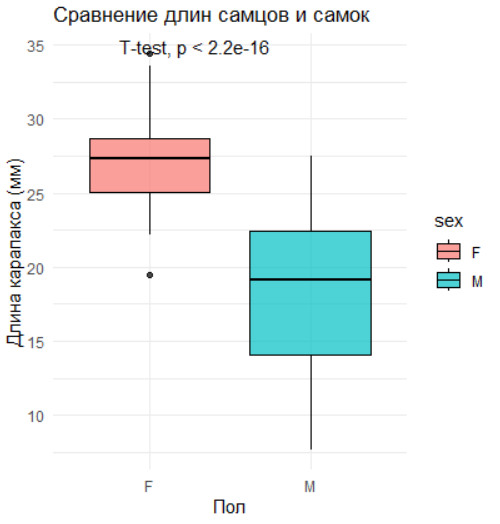
\includegraphics[width=0.6\linewidth,height=\textheight,keepaspectratio]{images/ttest_shrimp.PNG}

}

\caption{Рис. 1.10: Boxplot сравнения длин самцов и самок}

\end{figure}%

\subsubsection{\texorpdfstring{\textbf{Интерпретация
результатов}}{Интерпретация результатов}}\label{ux438ux43dux442ux435ux440ux43fux440ux435ux442ux430ux446ux438ux44f-ux440ux435ux437ux443ux43bux44cux442ux430ux442ux43eux432}

\begin{enumerate}
\def\labelenumi{\arabic{enumi}.}
\item
  Если p-value \textless{} 0.05, различия между группами статистически
  значимы.
\item
  Эффект размера помогает оценить биологическую важность различий.
  Например, если самки значительно крупнее самцов (d = 1.2), это может
  указывать на половой диморфизм, связанный с репродуктивной стратегией.

  \subsubsection{\texorpdfstring{\textbf{Пример полного анализа для
  веса}}{Пример полного анализа для веса}}\label{ux43fux440ux438ux43cux435ux440-ux43fux43eux43bux43dux43eux433ux43e-ux430ux43dux430ux43bux438ux437ux430-ux434ux43bux44f-ux432ux435ux441ux430}
\end{enumerate}

\begin{Shaded}
\begin{Highlighting}[]
\CommentTok{\# Полный анализ для веса  }
\NormalTok{weight\_analysis }\OtherTok{\textless{}{-}}\NormalTok{ data }\SpecialCharTok{\%\textgreater{}\%}  
  \FunctionTok{group\_by}\NormalTok{(sex) }\SpecialCharTok{\%\textgreater{}\%}  
  \FunctionTok{summarise}\NormalTok{(  }
    \AttributeTok{mean\_weight =} \FunctionTok{mean}\NormalTok{(weight),  }
    \AttributeTok{sd\_weight =} \FunctionTok{sd}\NormalTok{(weight),  }
    \AttributeTok{n =} \FunctionTok{n}\NormalTok{()  }
\NormalTok{  ) }\SpecialCharTok{\%\textgreater{}\%}  
  \FunctionTok{mutate}\NormalTok{(  }
    \AttributeTok{t\_test =} \FunctionTok{list}\NormalTok{(}\FunctionTok{t\_test}\NormalTok{(weight }\SpecialCharTok{\textasciitilde{}}\NormalTok{ sex, }\AttributeTok{data =}\NormalTok{ data)),  }
    \AttributeTok{cohens\_d =} \FunctionTok{list}\NormalTok{(}\FunctionTok{cohens\_d}\NormalTok{(weight }\SpecialCharTok{\textasciitilde{}}\NormalTok{ sex, }\AttributeTok{data =}\NormalTok{ data))  }
\NormalTok{  )  }

\CommentTok{\# Вывод результатов  }
\FunctionTok{print}\NormalTok{(weight\_analysis) }

\CommentTok{\# Распределение веса по полу}
\FunctionTok{ggplot}\NormalTok{(data, }\FunctionTok{aes}\NormalTok{(}\AttributeTok{x =} \FunctionTok{factor}\NormalTok{(sex), }\AttributeTok{y =}\NormalTok{ weight, }\AttributeTok{fill =} \FunctionTok{factor}\NormalTok{(sex))) }\SpecialCharTok{+}
  \FunctionTok{geom\_violin}\NormalTok{(}\AttributeTok{trim =} \ConstantTok{FALSE}\NormalTok{, }\AttributeTok{alpha =} \FloatTok{0.7}\NormalTok{) }\SpecialCharTok{+}
  \FunctionTok{geom\_boxplot}\NormalTok{(}\AttributeTok{width =} \FloatTok{0.2}\NormalTok{, }\AttributeTok{outlier.shape =} \ConstantTok{NA}\NormalTok{, }\AttributeTok{fill =} \StringTok{"white"}\NormalTok{) }\SpecialCharTok{+}
  \FunctionTok{labs}\NormalTok{(}\AttributeTok{title =} \StringTok{"Распределение веса по полу"}\NormalTok{, }\AttributeTok{x =} \StringTok{"Пол"}\NormalTok{, }\AttributeTok{y =} \StringTok{"Вес (г)"}\NormalTok{) }\SpecialCharTok{+}
  \FunctionTok{theme\_minimal}\NormalTok{()}
\end{Highlighting}
\end{Shaded}

\begin{figure}[H]

{\centering 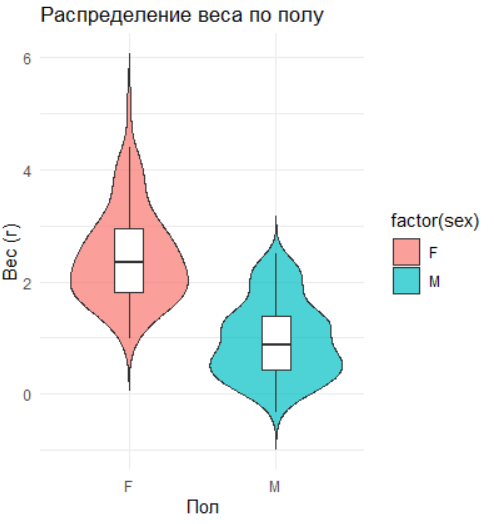
\includegraphics[width=0.6\linewidth,height=\textheight,keepaspectratio]{images/violin_shrimp.PNG}

}

\caption{Рис. 1.12: Violin plot для визуализации распределения веса}

\end{figure}%

\subsubsection{\texorpdfstring{\textbf{Выводы}}{Выводы}}\label{ux432ux44bux432ux43eux434ux44b}

\begin{enumerate}
\def\labelenumi{\arabic{enumi}.}
\item
  Используйте t-тест для нормальных данных и U-тест для ненормальных.
\item
  Дополните анализ оценкой эффекта размера для биологической
  интерпретации.
\item
  Визуализируйте различия с помощью boxplot или violin plot.
\end{enumerate}

\textbf{Рекомендации} :

\begin{itemize}
\item
  Для многомерных данных (например, одновременное сравнение длины, веса
  и возраста) применяйте MANOVA.
\item
  Если группы неоднородны (например, разный возрастной состав),
  используйте ковариационный анализ (ANCOVA).

  \subsection{\texorpdfstring{\textbf{Что делать, если тест на
  нормальность не пройден для одной из
  групп?}}{Что делать, если тест на нормальность не пройден для одной из групп?}}\label{ux447ux442ux43e-ux434ux435ux43bux430ux442ux44c-ux435ux441ux43bux438-ux442ux435ux441ux442-ux43dux430-ux43dux43eux440ux43cux430ux43bux44cux43dux43eux441ux442ux44c-ux43dux435-ux43fux440ux43eux439ux434ux435ux43d-ux434ux43bux44f-ux43eux434ux43dux43eux439-ux438ux437-ux433ux440ux443ux43fux43f}

  При сравнении количественных характеристик (например, длины карапакса
  у самцов и самок) важно учитывать, соответствуют ли данные нормальному
  распределению. Если тест на нормальность (например, Шапиро-Уилка)
  показывает значимое отклонение от нормальности для одной из групп, это
  влияет на выбор статистического теста и интерпретацию результатов.

  \subsubsection{\texorpdfstring{\textbf{Пример из нашего
  анализа}}{Пример из нашего анализа}}\label{ux43fux440ux438ux43cux435ux440-ux438ux437-ux43dux430ux448ux435ux433ux43e-ux430ux43dux430ux43bux438ux437ux430}

  Мы провели сравнение длины карапакса между самцами и самками:

  \begin{itemize}
  \item
    Для самцов: \textbf{\texttt{shapiro\_test(males\$length)}} → p-value
    = \textbf{0.000574} (нормальность отвергнута).
  \item
    Для самок: \textbf{\texttt{shapiro\_test(females\$length)}} →
    p-value = \textbf{0.891} (нормальность подтверждена).
  \end{itemize}

  Несмотря на это, мы применили как \textbf{t-тест} , так и
  \textbf{U-тест Манна-Уитни} :

  \begin{itemize}
  \item
    \textbf{t-тест} : p-value = 1.46e-40 (значимо).
  \item
    \textbf{U-тест} : p-value = 1.97e-27 (значимо).
  \item
    Коэффициент Коэна: d = 2.14 (большой эффект).
  \end{itemize}

  \subsubsection{\texorpdfstring{\textbf{Почему это
  работает?}}{Почему это работает?}}\label{ux43fux43eux447ux435ux43cux443-ux44dux442ux43e-ux440ux430ux431ux43eux442ux430ux435ux442}

  \begin{enumerate}
  \def\labelenumi{\arabic{enumi}.}
  \item
    \textbf{t-тест устойчив к умеренным отклонениям от нормальности} :

    \begin{itemize}
    \item
      При больших выборках (n \textgreater{} 30) центральная предельная
      теорема позволяет использовать t-тест даже при слабо выраженной
      асимметрии.
    \item
      В вашем случае выборка самцов (n = 149) достаточно велика, чтобы
      компенсировать отклонение от нормальности.
    \end{itemize}
  \item
    \textbf{U-тест Манна-Уитни --- непараметрическая альтернатива} :

    \begin{itemize}
    \item
      Этот тест не требует нормальности и сравнивает ранги, а не средние
      значения.
    \item
      Он подтверждает значимость различий, что усиливает доверие к
      выводу.
    \end{itemize}
  \item
    \textbf{Эффект размера (коэффициент Кобена)} :

    \begin{itemize}
    \tightlist
    \item
      d = 2.14 указывает на \textbf{большой эффект} , что важно для
      биологической интерпретации, даже если p-values значимы.
    \end{itemize}
  \end{enumerate}
\end{itemize}

\subsection{Сравнение параметров (линейные модели для оценки
межгрупповых
различий)}\label{ux441ux440ux430ux432ux43dux435ux43dux438ux435-ux43fux430ux440ux430ux43cux435ux442ux440ux43eux432-ux43bux438ux43dux435ux439ux43dux44bux435-ux43cux43eux434ux435ux43bux438-ux434ux43bux44f-ux43eux446ux435ux43dux43aux438-ux43cux435ux436ux433ux440ux443ux43fux43fux43eux432ux44bux445-ux440ux430ux437ux43bux438ux447ux438ux439}

Для сравнения параметров двух линейных моделей (например, скорости роста
самцов и самок) используем следующий подход.

\begin{Shaded}
\begin{Highlighting}[]
\CommentTok{\# Установка рабочей директории}
\FunctionTok{setwd}\NormalTok{(}\StringTok{"C:/TEXTBOOK/"}\NormalTok{)}

\CommentTok{\# Загрузка библиотек}
\FunctionTok{library}\NormalTok{(tidyverse)}
\FunctionTok{library}\NormalTok{(ggplot2)}
\FunctionTok{library}\NormalTok{(broom)}
\FunctionTok{library}\NormalTok{(knitr)}

\CommentTok{\# Загрузка данных}
\NormalTok{data }\OtherTok{\textless{}{-}} \FunctionTok{read\_csv}\NormalTok{(}\StringTok{"shrimp\_catch.csv"}\NormalTok{) }\SpecialCharTok{\%\textgreater{}\%}
  \FunctionTok{filter}\NormalTok{(}\SpecialCharTok{!}\NormalTok{id }\SpecialCharTok{\%in\%} \FunctionTok{c}\NormalTok{(}\DecValTok{10}\NormalTok{, }\DecValTok{50}\NormalTok{))  }\CommentTok{\# Удаление аномальных наблюдений}

\CommentTok{\# Фильтрация данных по полу}
\NormalTok{data\_male }\OtherTok{\textless{}{-}}\NormalTok{ data }\SpecialCharTok{\%\textgreater{}\%} \FunctionTok{filter}\NormalTok{(sex }\SpecialCharTok{==} \StringTok{"M"}\NormalTok{)}
\NormalTok{data\_female }\OtherTok{\textless{}{-}}\NormalTok{ data }\SpecialCharTok{\%\textgreater{}\%} \FunctionTok{filter}\NormalTok{(sex }\SpecialCharTok{==} \StringTok{"F"}\NormalTok{)}

\CommentTok{\# Построение моделей}
\NormalTok{model\_male }\OtherTok{\textless{}{-}} \FunctionTok{lm}\NormalTok{(length }\SpecialCharTok{\textasciitilde{}}\NormalTok{ age, }\AttributeTok{data =}\NormalTok{ data\_male)}
\NormalTok{model\_female }\OtherTok{\textless{}{-}} \FunctionTok{lm}\NormalTok{(length }\SpecialCharTok{\textasciitilde{}}\NormalTok{ age, }\AttributeTok{data =}\NormalTok{ data\_female)}

\FunctionTok{ggplot}\NormalTok{(data, }\FunctionTok{aes}\NormalTok{(age, length, }\AttributeTok{color =}\NormalTok{ sex)) }\SpecialCharTok{+}
  \FunctionTok{geom\_point}\NormalTok{(}\AttributeTok{alpha =} \FloatTok{0.5}\NormalTok{) }\SpecialCharTok{+}
  \FunctionTok{geom\_smooth}\NormalTok{(}\AttributeTok{method =} \StringTok{"lm"}\NormalTok{, }\AttributeTok{formula =}\NormalTok{ y }\SpecialCharTok{\textasciitilde{}}\NormalTok{ x) }\SpecialCharTok{+}
  \FunctionTok{scale\_color\_manual}\NormalTok{(}\AttributeTok{values =} \FunctionTok{c}\NormalTok{(}\StringTok{"\#E7B800"}\NormalTok{, }\StringTok{"\#00AFBB"}\NormalTok{)) }\SpecialCharTok{+}
  \FunctionTok{labs}\NormalTok{(}\AttributeTok{x =} \StringTok{"Возраст"}\NormalTok{, }\AttributeTok{y =} \StringTok{"Длина (мм)"}\NormalTok{) }\SpecialCharTok{+}
  \FunctionTok{theme\_minimal}\NormalTok{()}
\end{Highlighting}
\end{Shaded}

\begin{figure}[H]

{\centering 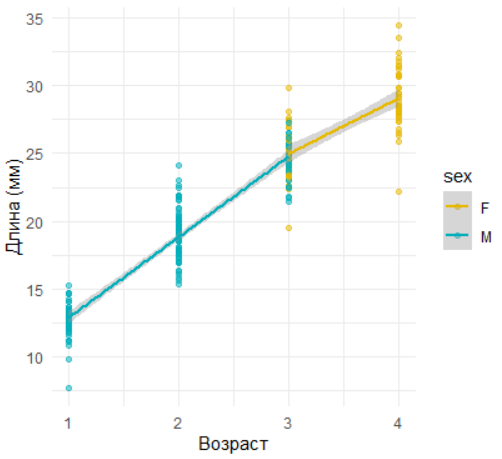
\includegraphics[width=0.6\linewidth,height=\textheight,keepaspectratio]{images/comparison_shrimp.PNG}

}

\caption{Рис. 1.15: Визуализация моделей}

\end{figure}%

\textbf{Метод 1: Объединенная модель с взаимодействиями}

\begin{Shaded}
\begin{Highlighting}[]
\CommentTok{\# Установка рабочей директории}
\NormalTok{joint\_model }\OtherTok{\textless{}{-}} \FunctionTok{lm}\NormalTok{(length }\SpecialCharTok{\textasciitilde{}}\NormalTok{ age }\SpecialCharTok{*}\NormalTok{ sex, }\AttributeTok{data =}\NormalTok{ data)}
\FunctionTok{summary}\NormalTok{(joint\_model) }\SpecialCharTok{\%\textgreater{}\%} 
\NormalTok{  broom}\SpecialCharTok{::}\FunctionTok{tidy}\NormalTok{() }\SpecialCharTok{\%\textgreater{}\%} 
  \FunctionTok{filter}\NormalTok{(term }\SpecialCharTok{==} \StringTok{"age:sexM"}\NormalTok{) }\SpecialCharTok{\%\textgreater{}\%} 
  \FunctionTok{kable}\NormalTok{(}\AttributeTok{caption =} \StringTok{"Проверка различия наклонов"}\NormalTok{, }\AttributeTok{digits =} \DecValTok{3}\NormalTok{)}
\end{Highlighting}
\end{Shaded}

\begin{Shaded}
\begin{Highlighting}[]
\NormalTok{Table}\SpecialCharTok{:}\NormalTok{ Проверка различия наклонов}

\SpecialCharTok{|}\NormalTok{term     }\SpecialCharTok{|}\NormalTok{ estimate}\SpecialCharTok{|}\NormalTok{ std.error}\SpecialCharTok{|}\NormalTok{ statistic}\SpecialCharTok{|}\NormalTok{ p.value}\SpecialCharTok{|}
\ErrorTok{|:}\SpecialCharTok{{-}{-}{-}{-}{-}{-}{-}{-}}\ErrorTok{|}\SpecialCharTok{{-}{-}{-}{-}{-}{-}{-}{-}}\ErrorTok{:|}\SpecialCharTok{{-}{-}{-}{-}{-}{-}{-}{-}{-}}\ErrorTok{:|}\SpecialCharTok{{-}{-}{-}{-}{-}{-}{-}{-}{-}}\ErrorTok{:|}\SpecialCharTok{{-}{-}{-}{-}{-}{-}{-}}\ErrorTok{:|}
\ErrorTok{|}\NormalTok{age}\SpecialCharTok{:}\NormalTok{sexM }\SpecialCharTok{|}     \FloatTok{1.86}\SpecialCharTok{|}     \FloatTok{0.459}\SpecialCharTok{|}     \FloatTok{4.053}\SpecialCharTok{|}       \DecValTok{0}\SpecialCharTok{|}
\ErrorTok{\textgreater{}} 
\end{Highlighting}
\end{Shaded}

\textbf{Интерпретация:}\\
Значимый коэффициент взаимодействия \textbf{\texttt{age:sexM}} (p
\textless{} 0.05) указывает на статистически значимые различия в
скорости роста между полами.

\textbf{Метод 2: Тест Вальда}

\begin{Shaded}
\begin{Highlighting}[]
\FunctionTok{library}\NormalTok{(car)}
\NormalTok{delta\_beta }\OtherTok{\textless{}{-}} \FunctionTok{coef}\NormalTok{(model\_male)[}\StringTok{"age"}\NormalTok{] }\SpecialCharTok{{-}} \FunctionTok{coef}\NormalTok{(model\_female)[}\StringTok{"age"}\NormalTok{]}
\NormalTok{se\_diff }\OtherTok{\textless{}{-}} \FunctionTok{sqrt}\NormalTok{(}\FunctionTok{vcov}\NormalTok{(model\_male)[}\StringTok{"age"}\NormalTok{,}\StringTok{"age"}\NormalTok{] }\SpecialCharTok{+} \FunctionTok{vcov}\NormalTok{(model\_female)[}\StringTok{"age"}\NormalTok{,}\StringTok{"age"}\NormalTok{])}
\NormalTok{z\_score }\OtherTok{\textless{}{-}}\NormalTok{ delta\_beta }\SpecialCharTok{/}\NormalTok{ se\_diff}
\NormalTok{p\_value }\OtherTok{\textless{}{-}} \DecValTok{2} \SpecialCharTok{*} \FunctionTok{pnorm}\NormalTok{(}\SpecialCharTok{{-}}\FunctionTok{abs}\NormalTok{(z\_score))}

\FunctionTok{cat}\NormalTok{(}\StringTok{"Разница коэффициентов:"}\NormalTok{, }\FunctionTok{round}\NormalTok{(delta\_beta, }\DecValTok{3}\NormalTok{), }
    \StringTok{"}\SpecialCharTok{\textbackslash{}n}\StringTok{Z{-}статистика:"}\NormalTok{, }\FunctionTok{round}\NormalTok{(z\_score, }\DecValTok{3}\NormalTok{),}
    \StringTok{"}\SpecialCharTok{\textbackslash{}n}\StringTok{p{-}value:"}\NormalTok{, }\FunctionTok{format.pval}\NormalTok{(p\_value, }\AttributeTok{digits =} \DecValTok{2}\NormalTok{))}


\NormalTok{comparison\_table }\OtherTok{\textless{}{-}} \FunctionTok{data.frame}\NormalTok{(}
\NormalTok{  Параметр }\OtherTok{=} \FunctionTok{c}\NormalTok{(}\StringTok{"Скорость роста самцов"}\NormalTok{, }\StringTok{"Скорость роста самок"}\NormalTok{, }\StringTok{"Разница"}\NormalTok{),}
\NormalTok{  Значение }\OtherTok{=} \FunctionTok{c}\NormalTok{(}
    \FunctionTok{round}\NormalTok{(}\FunctionTok{coef}\NormalTok{(model\_male)[}\StringTok{"age"}\NormalTok{], }\DecValTok{2}\NormalTok{),}
    \FunctionTok{round}\NormalTok{(}\FunctionTok{coef}\NormalTok{(model\_female)[}\StringTok{"age"}\NormalTok{], }\DecValTok{2}\NormalTok{),}
    \FunctionTok{round}\NormalTok{(delta\_beta, }\DecValTok{2}\NormalTok{)}
\NormalTok{  ),}
  \StringTok{\textasciigrave{}}\AttributeTok{p{-}value}\StringTok{\textasciigrave{}} \OtherTok{=} \FunctionTok{c}\NormalTok{(}
    \FunctionTok{format.pval}\NormalTok{(}\FunctionTok{summary}\NormalTok{(model\_male)}\SpecialCharTok{$}\NormalTok{coefficients[}\StringTok{"age"}\NormalTok{,}\DecValTok{4}\NormalTok{], }\AttributeTok{digits =} \DecValTok{2}\NormalTok{),}
    \FunctionTok{format.pval}\NormalTok{(}\FunctionTok{summary}\NormalTok{(model\_female)}\SpecialCharTok{$}\NormalTok{coefficients[}\StringTok{"age"}\NormalTok{,}\DecValTok{4}\NormalTok{], }\AttributeTok{digits =} \DecValTok{2}\NormalTok{),}
    \FunctionTok{format.pval}\NormalTok{(p\_value, }\AttributeTok{digits =} \DecValTok{2}\NormalTok{)}
\NormalTok{  )}
\NormalTok{)}
\FunctionTok{kable}\NormalTok{(comparison\_table, }\AttributeTok{caption =} \StringTok{"Сравнение коэффициентов роста"}\NormalTok{)}
\end{Highlighting}
\end{Shaded}

Вывод

\begin{Shaded}
\begin{Highlighting}[]
\SpecialCharTok{:}\NormalTok{ Сравнение коэффициентов роста}

\SpecialCharTok{|}\NormalTok{Параметр              }\SpecialCharTok{|}\NormalTok{ Значение}\SpecialCharTok{|}\NormalTok{p.value }\SpecialCharTok{|}
\ErrorTok{|:}\SpecialCharTok{{-}{-}{-}{-}{-}{-}{-}{-}{-}{-}{-}{-}{-}{-}{-}{-}{-}{-}{-}{-}{-}}\ErrorTok{|}\SpecialCharTok{{-}{-}{-}{-}{-}{-}{-}{-}}\ErrorTok{:|:}\SpecialCharTok{{-}{-}{-}{-}{-}{-}{-}}\ErrorTok{|}
\ErrorTok{|}\NormalTok{Скорость роста самцов }\SpecialCharTok{|}     \FloatTok{5.95}\SpecialCharTok{|}\ErrorTok{\textless{}}\FloatTok{2e{-}16}  \SpecialCharTok{|}
\ErrorTok{|}\NormalTok{Скорость роста самок  }\SpecialCharTok{|}     \FloatTok{4.09}\SpecialCharTok{|}\FloatTok{5.2e{-}13} \SpecialCharTok{|}
\ErrorTok{|}\NormalTok{Разница               }\SpecialCharTok{|}     \FloatTok{1.86}\SpecialCharTok{|}\FloatTok{0.00024} \SpecialCharTok{|}
\ErrorTok{\textgreater{}} 
\end{Highlighting}
\end{Shaded}

\textbf{Интерпретация:}\\
Значимая \emph{разница} (p \textless{} 0.05) указывает на статистически
значимые различия в скорости роста между полами.

\subsection{Сравнение
моделей}\label{ux441ux440ux430ux432ux43dux435ux43dux438ux435-ux43cux43eux434ux435ux43bux435ux439}

Одним из ключевых аспектов анализа биологических данных является
определение формы зависимости между переменными. В данном разделе мы
рассмотрим основы подбора модели зависимости между длиной и весом
креветок. Начиная с простой линейной модели, мы постепенно перейдем к
более сложным нелинейным моделям, чтобы продемонстрировать методику
выбора наилучшей модели. Cравним три модели --- линейную, полиномиальную
и степенную --- чтобы определить, какая из них наилучшим образом
описывает данные. Цель анализа --- найти математическую зависимость,
которая:

\begin{enumerate}
\def\labelenumi{\arabic{enumi}.}
\item
  Точно предсказывает вес креветки по её длине.
\item
  Имеет биологическую интерпретацию.
\item
  Минимизирует ошибку предсказания.
\end{enumerate}

\subsubsection{Модели и их
параметры}\label{ux43cux43eux434ux435ux43bux438-ux438-ux438ux445-ux43fux430ux440ux430ux43cux435ux442ux440ux44b}

\begin{enumerate}
\def\labelenumi{\arabic{enumi}.}
\tightlist
\item
  \textbf{Линейная}:
  \(\text{weight} = \beta_0 + \beta_1\cdot\text{length}\)
\item
  \textbf{Полиномиальная 3-й степени}:
  \(\text{weight} = \beta_0 + \beta_1\cdot\text{length} + \beta_2\cdot\text{length}^2 + \beta_3\cdot\text{length}^3\)
\item
  \textbf{Степенная}: \(\text{weight} = a\cdot\text{length}^b\)
\end{enumerate}

\subsubsection{Метрики}\label{ux43cux435ux442ux440ux438ux43aux438}

\begin{itemize}
\tightlist
\item
  \textbf{R²} - (коэффициент детерминации): чем ближе к 1, тем лучше
  модель объясняет данные.
\item
  \textbf{AIC} -(информационный критерий Акаике): чем меньше значение,
  тем лучше модель с учётом её сложности.
\end{itemize}

\subsubsection{\texorpdfstring{\textbf{Результаты}}{Результаты}}\label{ux440ux435ux437ux443ux43bux44cux442ux430ux442ux44b}

\paragraph{\texorpdfstring{\textbf{1. Линейная
модель}}{1. Линейная модель}}\label{ux43bux438ux43dux435ux439ux43dux430ux44f-ux43cux43eux434ux435ux43bux44c}

\begin{Shaded}
\begin{Highlighting}[]
\NormalTok{Coefficients}\SpecialCharTok{:}
\NormalTok{             Estimate Std. Error t value }\FunctionTok{Pr}\NormalTok{(}\SpecialCharTok{\textgreater{}}\ErrorTok{|}\NormalTok{t}\SpecialCharTok{|}\NormalTok{)    }
\NormalTok{(Intercept) }\SpecialCharTok{{-}}\FloatTok{2.115}      \FloatTok{0.085}     \SpecialCharTok{{-}}\FloatTok{24.86}   \SpecialCharTok{\textless{}}\FloatTok{2e{-}16} \SpecialCharTok{**}\ErrorTok{*}
\NormalTok{length       }\FloatTok{0.1665}     \FloatTok{0.0038}    \FloatTok{43.71}    \SpecialCharTok{\textless{}}\FloatTok{2e{-}16} \SpecialCharTok{**}\ErrorTok{*}
\end{Highlighting}
\end{Shaded}

\begin{itemize}
\item
  \textbf{R² = 0.894}
\item
  \textbf{AIC = 148.02}
\end{itemize}

\begin{figure}[H]

{\centering 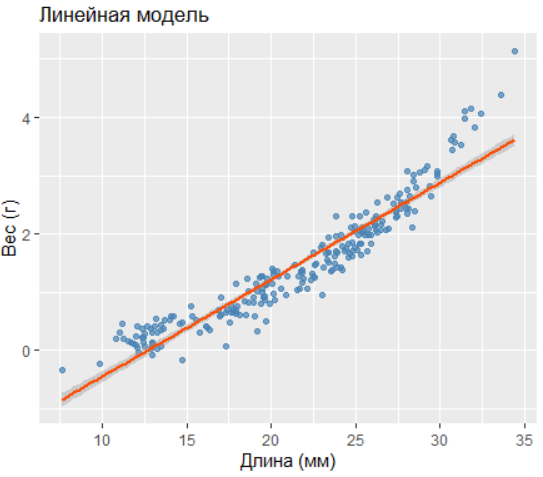
\includegraphics[width=0.6\linewidth,height=\textheight,keepaspectratio]{images/linear_shrimp.PNG}

}

\caption{Рис. 1.5: Линейная модель}

\end{figure}%

\paragraph{\texorpdfstring{\textbf{2. Полиномиальная
модель}}{2. Полиномиальная модель}}\label{ux43fux43eux43bux438ux43dux43eux43cux438ux430ux43bux44cux43dux430ux44f-ux43cux43eux434ux435ux43bux44c}

\begin{Shaded}
\begin{Highlighting}[]
\NormalTok{Coefficients}\SpecialCharTok{:}
\NormalTok{                 Estimate Std. Error t value }\FunctionTok{Pr}\NormalTok{(}\SpecialCharTok{\textgreater{}}\ErrorTok{|}\NormalTok{t}\SpecialCharTok{|}\NormalTok{)    }
\FunctionTok{poly}\NormalTok{(length,}\DecValTok{3}\NormalTok{)}\DecValTok{1}  \FloatTok{14.5038}    \FloatTok{0.2127}    \FloatTok{68.18}   \SpecialCharTok{\textless{}}\FloatTok{2e{-}16} \SpecialCharTok{**}\ErrorTok{*}
\FunctionTok{poly}\NormalTok{(length,}\DecValTok{3}\NormalTok{)}\DecValTok{2}   \FloatTok{3.7209}    \FloatTok{0.2127}    \FloatTok{17.49}   \SpecialCharTok{\textless{}}\FloatTok{2e{-}16} \SpecialCharTok{**}\ErrorTok{*}
\FunctionTok{poly}\NormalTok{(length,}\DecValTok{3}\NormalTok{)}\DecValTok{3}   \FloatTok{0.9526}    \FloatTok{0.2127}     \FloatTok{4.48}  \FloatTok{1.2e{-}05} \SpecialCharTok{**}\ErrorTok{*}
\end{Highlighting}
\end{Shaded}

\begin{itemize}
\item
  \textbf{R² = 0.957}
\item
  \textbf{AIC = -52.80}
\end{itemize}

\begin{figure}[H]

{\centering 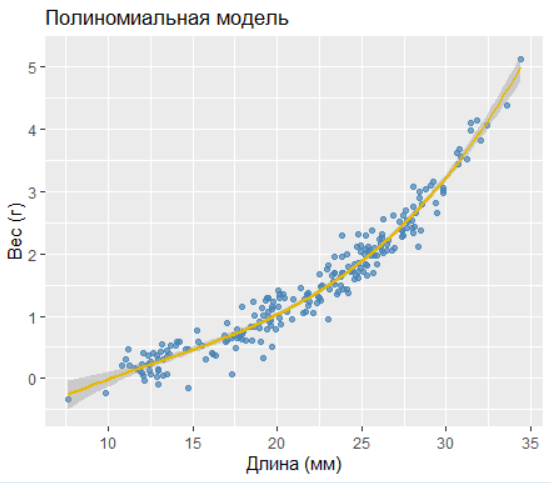
\includegraphics[width=0.6\linewidth,height=\textheight,keepaspectratio]{images/poly_shrimp.PNG}

}

\caption{Рис. 1.5: Полиномиальная модель}

\end{figure}%

\paragraph{\texorpdfstring{\textbf{3. Степенная
модель}}{3. Степенная модель}}\label{ux441ux442ux435ux43fux435ux43dux43dux430ux44f-ux43cux43eux434ux435ux43bux44c}

\begin{Shaded}
\begin{Highlighting}[]
\NormalTok{Parameters}\SpecialCharTok{:}
\NormalTok{   Estimate Std. Error t value }\FunctionTok{Pr}\NormalTok{(}\SpecialCharTok{\textgreater{}}\ErrorTok{|}\NormalTok{t}\SpecialCharTok{|}\NormalTok{)    }
\NormalTok{a }\FloatTok{0.000157}   \FloatTok{0.000028}    \FloatTok{5.60}  \FloatTok{6.3e{-}08} \SpecialCharTok{**}\ErrorTok{*}
\NormalTok{b }\FloatTok{2.920160}   \FloatTok{0.054102}   \FloatTok{53.98}   \SpecialCharTok{\textless{}}\FloatTok{2e{-}16} \SpecialCharTok{**}\ErrorTok{*}
\end{Highlighting}
\end{Shaded}

\begin{itemize}
\item
  \textbf{R² = 0.955}
\item
  \textbf{AIC = -48.43} \begin{center}
  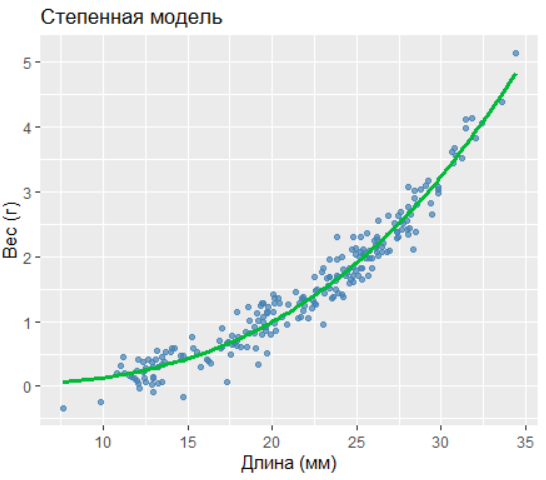
\includegraphics[width=0.6\linewidth,height=\textheight,keepaspectratio]{images/power_shrimp.PNG}
  \end{center}
\end{itemize}

\subsubsection{\texorpdfstring{\textbf{3. Сравнение
моделей}}{3. Сравнение моделей}}\label{ux441ux440ux430ux432ux43dux435ux43dux438ux435-ux43cux43eux434ux435ux43bux435ux439-1}

\begin{longtable}[]{@{}lll@{}}
\toprule\noalign{}
\textbf{Модель} & \textbf{R²} & \textbf{AIC} \\
\midrule\noalign{}
\endhead
\bottomrule\noalign{}
\endlastfoot
Линейная & 0.894 & 148.02 \\
Полиномиальная & 0.957 & -52.80 \\
Степенная & 0.955 & -48.43 \\
\end{longtable}

\textbf{Выводы:}

\begin{enumerate}
\def\labelenumi{\arabic{enumi}.}
\item
  \textbf{Полиномиальная модель} демонстрирует наилучшие показатели
  (максимальный R² и минимальный AIC).
\item
  \textbf{Степенная модель} близка по качеству, но её параметр
  \emph{b}≈2.92 близок к биологически ожидаемому значению 3 (вес
  пропорционален объёму).
\item
  \textbf{Линейная модель} существенно уступает по точности.
\end{enumerate}

\subsubsection{\texorpdfstring{\textbf{4.
Рекомендации}}{4. Рекомендации}}\label{ux440ux435ux43aux43eux43cux435ux43dux434ux430ux446ux438ux438}

\begin{itemize}
\item
  \textbf{Для прогнозирования} используйте полиномиальную модель, так
  как она минимизирует ошибку.
\item
  \textbf{Для биологической интерпретации} предпочтительна степенная
  модель: weight∝length\textsuperscript{2.92}.
\item
  \textbf{Избегайте переобучения:} Полиномиальные модели высокой степени
  могут терять интерпретируемость.
\end{itemize}

\subsubsection{\texorpdfstring{\textbf{5. Визуализация
остатков}}{5. Визуализация остатков}}\label{ux432ux438ux437ux443ux430ux43bux438ux437ux430ux446ux438ux44f-ux43eux441ux442ux430ux442ux43aux43eux432}

Остатки степенной модели распределены равномерно, что подтверждает её
адекватность: \begin{center}
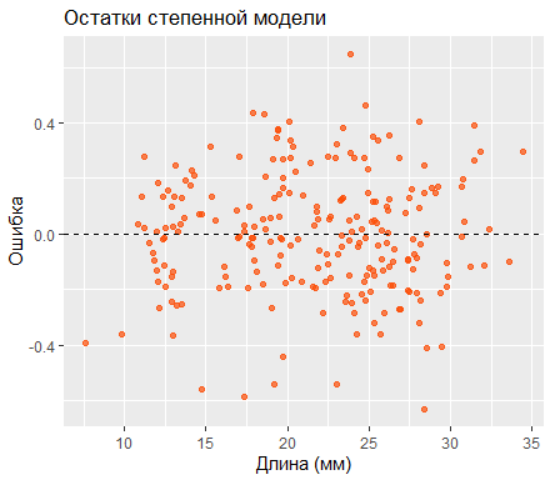
\includegraphics[width=0.6\linewidth,height=\textheight,keepaspectratio]{images/residuals_shrimp.PNG}
\end{center}

\subsubsection{\texorpdfstring{\textbf{Заключение}}{Заключение}}\label{ux437ux430ux43aux43bux44eux447ux435ux43dux438ux435}

Для анализа зависимости веса от длины северной креветки
\textbf{рекомендуется}:

\begin{enumerate}
\def\labelenumi{\arabic{enumi}.}
\item
  \textbf{Полиномиальная модель} --- для задач, требующих максимальной
  точности.
\item
  \textbf{Степенная модель} --- для интерпретации биологических
  закономерностей.
\end{enumerate}

Скрипт вышеописанных событий:

\begin{Shaded}
\begin{Highlighting}[]
\CommentTok{\# Установка рабочей директории}
\FunctionTok{setwd}\NormalTok{(}\StringTok{"C:/TEXTBOOK/"}\NormalTok{)}

\CommentTok{\# Загрузка библиотек}
\FunctionTok{library}\NormalTok{(tidyverse)}
\FunctionTok{library}\NormalTok{(ggplot2)}

\CommentTok{\# Загрузка данных}
\NormalTok{data }\OtherTok{\textless{}{-}} \FunctionTok{read\_csv}\NormalTok{(}\StringTok{"shrimp\_catch.csv"}\NormalTok{) }\SpecialCharTok{\%\textgreater{}\%}
  \FunctionTok{filter}\NormalTok{(}\SpecialCharTok{!}\NormalTok{id }\SpecialCharTok{\%in\%} \FunctionTok{c}\NormalTok{(}\DecValTok{10}\NormalTok{, }\DecValTok{50}\NormalTok{))  }\CommentTok{\# Удаление аномальных наблюдений}

\CommentTok{\# Проверка структуры}
\FunctionTok{glimpse}\NormalTok{(data)}

\CommentTok{\# Линейная модель: вес \textasciitilde{} длина}
\NormalTok{model\_linear }\OtherTok{\textless{}{-}} \FunctionTok{lm}\NormalTok{(weight }\SpecialCharTok{\textasciitilde{}}\NormalTok{ length, }\AttributeTok{data =}\NormalTok{ data)}
\FunctionTok{summary}\NormalTok{(model\_linear)}

\CommentTok{\# Визуализация}
\FunctionTok{ggplot}\NormalTok{(data, }\FunctionTok{aes}\NormalTok{(}\AttributeTok{x =}\NormalTok{ length, }\AttributeTok{y =}\NormalTok{ weight)) }\SpecialCharTok{+}
  \FunctionTok{geom\_point}\NormalTok{(}\AttributeTok{color =} \StringTok{"steelblue"}\NormalTok{, }\AttributeTok{alpha =} \FloatTok{0.7}\NormalTok{) }\SpecialCharTok{+}
  \FunctionTok{geom\_smooth}\NormalTok{(}\AttributeTok{method =} \StringTok{"lm"}\NormalTok{, }\AttributeTok{color =} \StringTok{"\#FC4E07"}\NormalTok{) }\SpecialCharTok{+}
  \FunctionTok{labs}\NormalTok{(}\AttributeTok{title =} \StringTok{"Линейная модель"}\NormalTok{, }\AttributeTok{x =} \StringTok{"Длина (мм)"}\NormalTok{, }\AttributeTok{y =} \StringTok{"Вес (г)"}\NormalTok{)}


\CommentTok{\# Полиномиальная модель: вес \textasciitilde{} длина + длина? + длина?}
\NormalTok{model\_poly }\OtherTok{\textless{}{-}} \FunctionTok{lm}\NormalTok{(weight }\SpecialCharTok{\textasciitilde{}} \FunctionTok{poly}\NormalTok{(length, }\DecValTok{3}\NormalTok{), }\AttributeTok{data =}\NormalTok{ data)}
\FunctionTok{summary}\NormalTok{(model\_poly)}

\CommentTok{\# Визуализация}
\FunctionTok{ggplot}\NormalTok{(data, }\FunctionTok{aes}\NormalTok{(}\AttributeTok{x =}\NormalTok{ length, }\AttributeTok{y =}\NormalTok{ weight)) }\SpecialCharTok{+}
  \FunctionTok{geom\_point}\NormalTok{(}\AttributeTok{color =} \StringTok{"steelblue"}\NormalTok{, }\AttributeTok{alpha =} \FloatTok{0.7}\NormalTok{) }\SpecialCharTok{+}
  \FunctionTok{geom\_smooth}\NormalTok{(}\AttributeTok{method =} \StringTok{"lm"}\NormalTok{, }\AttributeTok{formula =}\NormalTok{ y }\SpecialCharTok{\textasciitilde{}} \FunctionTok{poly}\NormalTok{(x, }\DecValTok{3}\NormalTok{), }\AttributeTok{color =} \StringTok{"\#E7B800"}\NormalTok{) }\SpecialCharTok{+}
  \FunctionTok{labs}\NormalTok{(}\AttributeTok{title =} \StringTok{"Полиномиальная модель"}\NormalTok{, }\AttributeTok{x =} \StringTok{"Длина (мм)"}\NormalTok{, }\AttributeTok{y =} \StringTok{"Вес (г)"}\NormalTok{)}


\CommentTok{\# Степенная модель: вес \textasciitilde{} длина\^{}k (k подбирается)}
\NormalTok{model\_power }\OtherTok{\textless{}{-}} \FunctionTok{nls}\NormalTok{(weight }\SpecialCharTok{\textasciitilde{}}\NormalTok{ a }\SpecialCharTok{*}\NormalTok{ length}\SpecialCharTok{\^{}}\NormalTok{b, }
                   \AttributeTok{data =}\NormalTok{ data, }
                   \AttributeTok{start =} \FunctionTok{list}\NormalTok{(}\AttributeTok{a =} \FloatTok{0.001}\NormalTok{, }\AttributeTok{b =} \DecValTok{3}\NormalTok{))  }\CommentTok{\# Начальные значения}
\FunctionTok{summary}\NormalTok{(model\_power)}

\CommentTok{\# Визуализация}
\NormalTok{data}\SpecialCharTok{$}\NormalTok{pred\_power }\OtherTok{\textless{}{-}} \FunctionTok{predict}\NormalTok{(model\_power)}
\FunctionTok{ggplot}\NormalTok{(data, }\FunctionTok{aes}\NormalTok{(}\AttributeTok{x =}\NormalTok{ length, }\AttributeTok{y =}\NormalTok{ weight)) }\SpecialCharTok{+}
  \FunctionTok{geom\_point}\NormalTok{(}\AttributeTok{color =} \StringTok{"steelblue"}\NormalTok{, }\AttributeTok{alpha =} \FloatTok{0.7}\NormalTok{) }\SpecialCharTok{+}
  \FunctionTok{geom\_line}\NormalTok{(}\FunctionTok{aes}\NormalTok{(}\AttributeTok{y =}\NormalTok{ pred\_power), }\AttributeTok{color =} \StringTok{"\#00BA38"}\NormalTok{, }\AttributeTok{linewidth =} \FloatTok{1.2}\NormalTok{) }\SpecialCharTok{+}
  \FunctionTok{labs}\NormalTok{(}\AttributeTok{title =} \StringTok{"Степенная модель"}\NormalTok{, }\AttributeTok{x =} \StringTok{"Длина (мм)"}\NormalTok{, }\AttributeTok{y =} \StringTok{"Вес (г)"}\NormalTok{)}

\CommentTok{\# Расчет AIC}
\FunctionTok{AIC}\NormalTok{(model\_linear, model\_poly, model\_power)}

\CommentTok{\# Расчет R?}
\NormalTok{r2\_linear }\OtherTok{\textless{}{-}} \FunctionTok{summary}\NormalTok{(model\_linear)}\SpecialCharTok{$}\NormalTok{r.squared}
\NormalTok{r2\_poly }\OtherTok{\textless{}{-}} \FunctionTok{summary}\NormalTok{(model\_poly)}\SpecialCharTok{$}\NormalTok{r.squared}
\NormalTok{r2\_power }\OtherTok{\textless{}{-}} \DecValTok{1} \SpecialCharTok{{-}} \FunctionTok{sum}\NormalTok{(}\FunctionTok{residuals}\NormalTok{(model\_power)}\SpecialCharTok{\^{}}\DecValTok{2}\NormalTok{) }\SpecialCharTok{/} \FunctionTok{sum}\NormalTok{((data}\SpecialCharTok{$}\NormalTok{weight }\SpecialCharTok{{-}} \FunctionTok{mean}\NormalTok{(data}\SpecialCharTok{$}\NormalTok{weight))}\SpecialCharTok{\^{}}\DecValTok{2}\NormalTok{)}

\CommentTok{\# Создание таблицы сравнения моделей}
\NormalTok{comparison\_table }\OtherTok{\textless{}{-}} \FunctionTok{data.frame}\NormalTok{(}
\NormalTok{  Модель }\OtherTok{=} \FunctionTok{c}\NormalTok{(}\StringTok{"Линейная"}\NormalTok{, }\StringTok{"Полиномиальная"}\NormalTok{, }\StringTok{"Степенная"}\NormalTok{),}
  \AttributeTok{R\_square =} \FunctionTok{c}\NormalTok{(r2\_linear, r2\_poly, r2\_power),}
  \AttributeTok{AIC =} \FunctionTok{c}\NormalTok{(}\FunctionTok{AIC}\NormalTok{(model\_linear), }\FunctionTok{AIC}\NormalTok{(model\_poly), }\FunctionTok{AIC}\NormalTok{(model\_power))}
\NormalTok{)}

\CommentTok{\# Вывод таблицы}
\FunctionTok{print}\NormalTok{(comparison\_table)}

\CommentTok{\# Остатки для степенной модели}
\NormalTok{data}\SpecialCharTok{$}\NormalTok{residuals }\OtherTok{\textless{}{-}} \FunctionTok{residuals}\NormalTok{(model\_power)}

\FunctionTok{ggplot}\NormalTok{(data, }\FunctionTok{aes}\NormalTok{(}\AttributeTok{x =}\NormalTok{ length, }\AttributeTok{y =}\NormalTok{ residuals)) }\SpecialCharTok{+}
  \FunctionTok{geom\_point}\NormalTok{(}\AttributeTok{color =} \StringTok{"\#FC4E07"}\NormalTok{, }\AttributeTok{alpha =} \FloatTok{0.7}\NormalTok{) }\SpecialCharTok{+}
  \FunctionTok{geom\_hline}\NormalTok{(}\AttributeTok{yintercept =} \DecValTok{0}\NormalTok{, }\AttributeTok{linetype =} \StringTok{"dashed"}\NormalTok{) }\SpecialCharTok{+}
  \FunctionTok{labs}\NormalTok{(}\AttributeTok{title =} \StringTok{"Остатки степенной модели"}\NormalTok{, }\AttributeTok{x =} \StringTok{"Длина (мм)"}\NormalTok{, }\AttributeTok{y =} \StringTok{"Ошибка"}\NormalTok{)}
\end{Highlighting}
\end{Shaded}

\bookmarksetup{startatroot}

\chapter{Введение в
картографию}\label{ux432ux432ux435ux434ux435ux43dux438ux435-ux432-ux43aux430ux440ux442ux43eux433ux440ux430ux444ux438ux44e}

\section{Введение}\label{ux432ux432ux435ux434ux435ux43dux438ux435-1}

Вступительное слово

\section{Раздел}\label{ux440ux430ux437ux434ux435ux43b}

Текст. Текст. Текст.

\section{Раздел}\label{ux440ux430ux437ux434ux435ux43b-1}

Текст. Текст. Текст.

\section{Выявление
аутлайеров}\label{ux432ux44bux44fux432ux43bux435ux43dux438ux435-ux430ux443ux442ux43bux430ux439ux435ux440ux43eux432}

Текст. Текст. Текст.

\bookmarksetup{startatroot}

\chapter{От регрессии и до нейронных
сетей}\label{ux43eux442-ux440ux435ux433ux440ux435ux441ux441ux438ux438-ux438-ux434ux43e-ux43dux435ux439ux440ux43eux43dux43dux44bux445-ux441ux435ux442ux435ux439}

\section{Введение}\label{ux432ux432ux435ux434ux435ux43dux438ux435-2}

\section{Загрузка данных и первичный
осмотр}\label{ux437ux430ux433ux440ux443ux437ux43aux430-ux434ux430ux43dux43dux44bux445-ux438-ux43fux435ux440ux432ux438ux447ux43dux44bux439-ux43eux441ux43cux43eux442ux440-1}

Текст. Текст. Текст.

\section{Описательная статистика и
визуализация}\label{ux43eux43fux438ux441ux430ux442ux435ux43bux44cux43dux430ux44f-ux441ux442ux430ux442ux438ux441ux442ux438ux43aux430-ux438-ux432ux438ux437ux443ux430ux43bux438ux437ux430ux446ux438ux44f-1}

Текст. Текст. Текст.

\bookmarksetup{startatroot}

\chapter{SDM - Модели пространственного распределения
видов}\label{sdm---ux43cux43eux434ux435ux43bux438-ux43fux440ux43eux441ux442ux440ux430ux43dux441ux442ux432ux435ux43dux43dux43eux433ux43e-ux440ux430ux441ux43fux440ux435ux434ux435ux43bux435ux43dux438ux44f-ux432ux438ux434ux43eux432}

\section{Введение}\label{ux432ux432ux435ux434ux435ux43dux438ux435-3}

\section{Загрузка данных и первичный
осмотр}\label{ux437ux430ux433ux440ux443ux437ux43aux430-ux434ux430ux43dux43dux44bux445-ux438-ux43fux435ux440ux432ux438ux447ux43dux44bux439-ux43eux441ux43cux43eux442ux440-2}

Текст. Текст. Текст.

\section{Описательная статистика и
визуализация}\label{ux43eux43fux438ux441ux430ux442ux435ux43bux44cux43dux430ux44f-ux441ux442ux430ux442ux438ux441ux442ux438ux43aux430-ux438-ux432ux438ux437ux443ux430ux43bux438ux437ux430ux446ux438ux44f-2}

Текст. Текст. Текст.

\bookmarksetup{startatroot}

\chapter{Основы
геостатистики}\label{ux43eux441ux43dux43eux432ux44b-ux433ux435ux43eux441ux442ux430ux442ux438ux441ux442ux438ux43aux438}

\section{Введение}\label{ux432ux432ux435ux434ux435ux43dux438ux435-4}

\section{Загрузка данных и первичный
осмотр}\label{ux437ux430ux433ux440ux443ux437ux43aux430-ux434ux430ux43dux43dux44bux445-ux438-ux43fux435ux440ux432ux438ux447ux43dux44bux439-ux43eux441ux43cux43eux442ux440-3}

Текст. Текст. Текст.

\section{Описательная статистика и
визуализация}\label{ux43eux43fux438ux441ux430ux442ux435ux43bux44cux43dux430ux44f-ux441ux442ux430ux442ux438ux441ux442ux438ux43aux430-ux438-ux432ux438ux437ux443ux430ux43bux438ux437ux430ux446ux438ux44f-3}

Текст. Текст. Текст.

\bookmarksetup{startatroot}

\chapter{Байесовский
подход}\label{ux431ux430ux439ux435ux441ux43eux432ux441ux43aux438ux439-ux43fux43eux434ux445ux43eux434}

\section{Введение}\label{ux432ux432ux435ux434ux435ux43dux438ux435-5}

\section{Загрузка данных и первичный
осмотр}\label{ux437ux430ux433ux440ux443ux437ux43aux430-ux434ux430ux43dux43dux44bux445-ux438-ux43fux435ux440ux432ux438ux447ux43dux44bux439-ux43eux441ux43cux43eux442ux440-4}

Текст. Текст. Текст.

\section{Описательная статистика и
визуализация}\label{ux43eux43fux438ux441ux430ux442ux435ux43bux44cux43dux430ux44f-ux441ux442ux430ux442ux438ux441ux442ux438ux43aux430-ux438-ux432ux438ux437ux443ux430ux43bux438ux437ux430ux446ux438ux44f-4}

Текст. Текст. Текст.

\bookmarksetup{startatroot}

\chapter{Продукционные
модели}\label{ux43fux440ux43eux434ux443ux43aux446ux438ux43eux43dux43dux44bux435-ux43cux43eux434ux435ux43bux438}

\section{Введение}\label{ux432ux432ux435ux434ux435ux43dux438ux435-6}

\section{Загрузка данных и первичный
осмотр}\label{ux437ux430ux433ux440ux443ux437ux43aux430-ux434ux430ux43dux43dux44bux445-ux438-ux43fux435ux440ux432ux438ux447ux43dux44bux439-ux43eux441ux43cux43eux442ux440-5}

Текст. Текст. Текст.

\section{Описательная статистика и
визуализация}\label{ux43eux43fux438ux441ux430ux442ux435ux43bux44cux43dux430ux44f-ux441ux442ux430ux442ux438ux441ux442ux438ux43aux430-ux438-ux432ux438ux437ux443ux430ux43bux438ux437ux430ux446ux438ux44f-5}

Текст. Текст. Текст.

\bookmarksetup{startatroot}

\chapter{Введение в
прогнозирование}\label{ux432ux432ux435ux434ux435ux43dux438ux435-ux432-ux43fux440ux43eux433ux43dux43eux437ux438ux440ux43eux432ux430ux43dux438ux435}

\section{Введение}\label{ux432ux432ux435ux434ux435ux43dux438ux435-7}

\section{Загрузка данных и первичный
осмотр}\label{ux437ux430ux433ux440ux443ux437ux43aux430-ux434ux430ux43dux43dux44bux445-ux438-ux43fux435ux440ux432ux438ux447ux43dux44bux439-ux43eux441ux43cux43eux442ux440-6}

Текст. Текст. Текст.

\section{Описательная статистика и
визуализация}\label{ux43eux43fux438ux441ux430ux442ux435ux43bux44cux43dux430ux44f-ux441ux442ux430ux442ux438ux441ux442ux438ux43aux430-ux438-ux432ux438ux437ux443ux430ux43bux438ux437ux430ux446ux438ux44f-6}

Текст. Текст. Текст.

\bookmarksetup{startatroot}

\chapter{ПРП и стратегии
управления}\label{ux43fux440ux43f-ux438-ux441ux442ux440ux430ux442ux435ux433ux438ux438-ux443ux43fux440ux430ux432ux43bux435ux43dux438ux44f}

\section{Введение}\label{ux432ux432ux435ux434ux435ux43dux438ux435-8}

\section{Загрузка данных и первичный
осмотр}\label{ux437ux430ux433ux440ux443ux437ux43aux430-ux434ux430ux43dux43dux44bux445-ux438-ux43fux435ux440ux432ux438ux447ux43dux44bux439-ux43eux441ux43cux43eux442ux440-7}

Текст. Текст. Текст.

\section{Описательная статистика и
визуализация}\label{ux43eux43fux438ux441ux430ux442ux435ux43bux44cux43dux430ux44f-ux441ux442ux430ux442ux438ux441ux442ux438ux43aux430-ux438-ux432ux438ux437ux443ux430ux43bux438ux437ux430ux446ux438ux44f-7}

Текст. Текст. Текст.

\bookmarksetup{startatroot}

\chapter*{References}\label{references}
\addcontentsline{toc}{chapter}{References}

\markboth{References}{References}

\phantomsection\label{refs}




\end{document}
